\documentclass[12pt]{report}
% pre\'ambulo

\usepackage{lmodern}
\usepackage[T1]{fontenc}
\usepackage[spanish, activeacute, es-tabla]{babel}
\usepackage{mathtools}
\usepackage[utf8]{inputenc}
\usepackage{cite}
\usepackage{graphicx}
\usepackage{float}
\usepackage{stackrel}
\usepackage{enumerate}
\usepackage{multirow}
\usepackage{wallpaper}
\usepackage{pdflscape}
\usepackage{geometry}
\usepackage{hyperref}
\usepackage{listings}
\graphicspath{ {./imagenes/} }


\begin{document}

\begingroup
\begin{titlepage}
    %\newgeometry{left=0cm,top=0cm,bottom=0cm, right=0cm}
    \AddToShipoutPicture*{\put(0,0){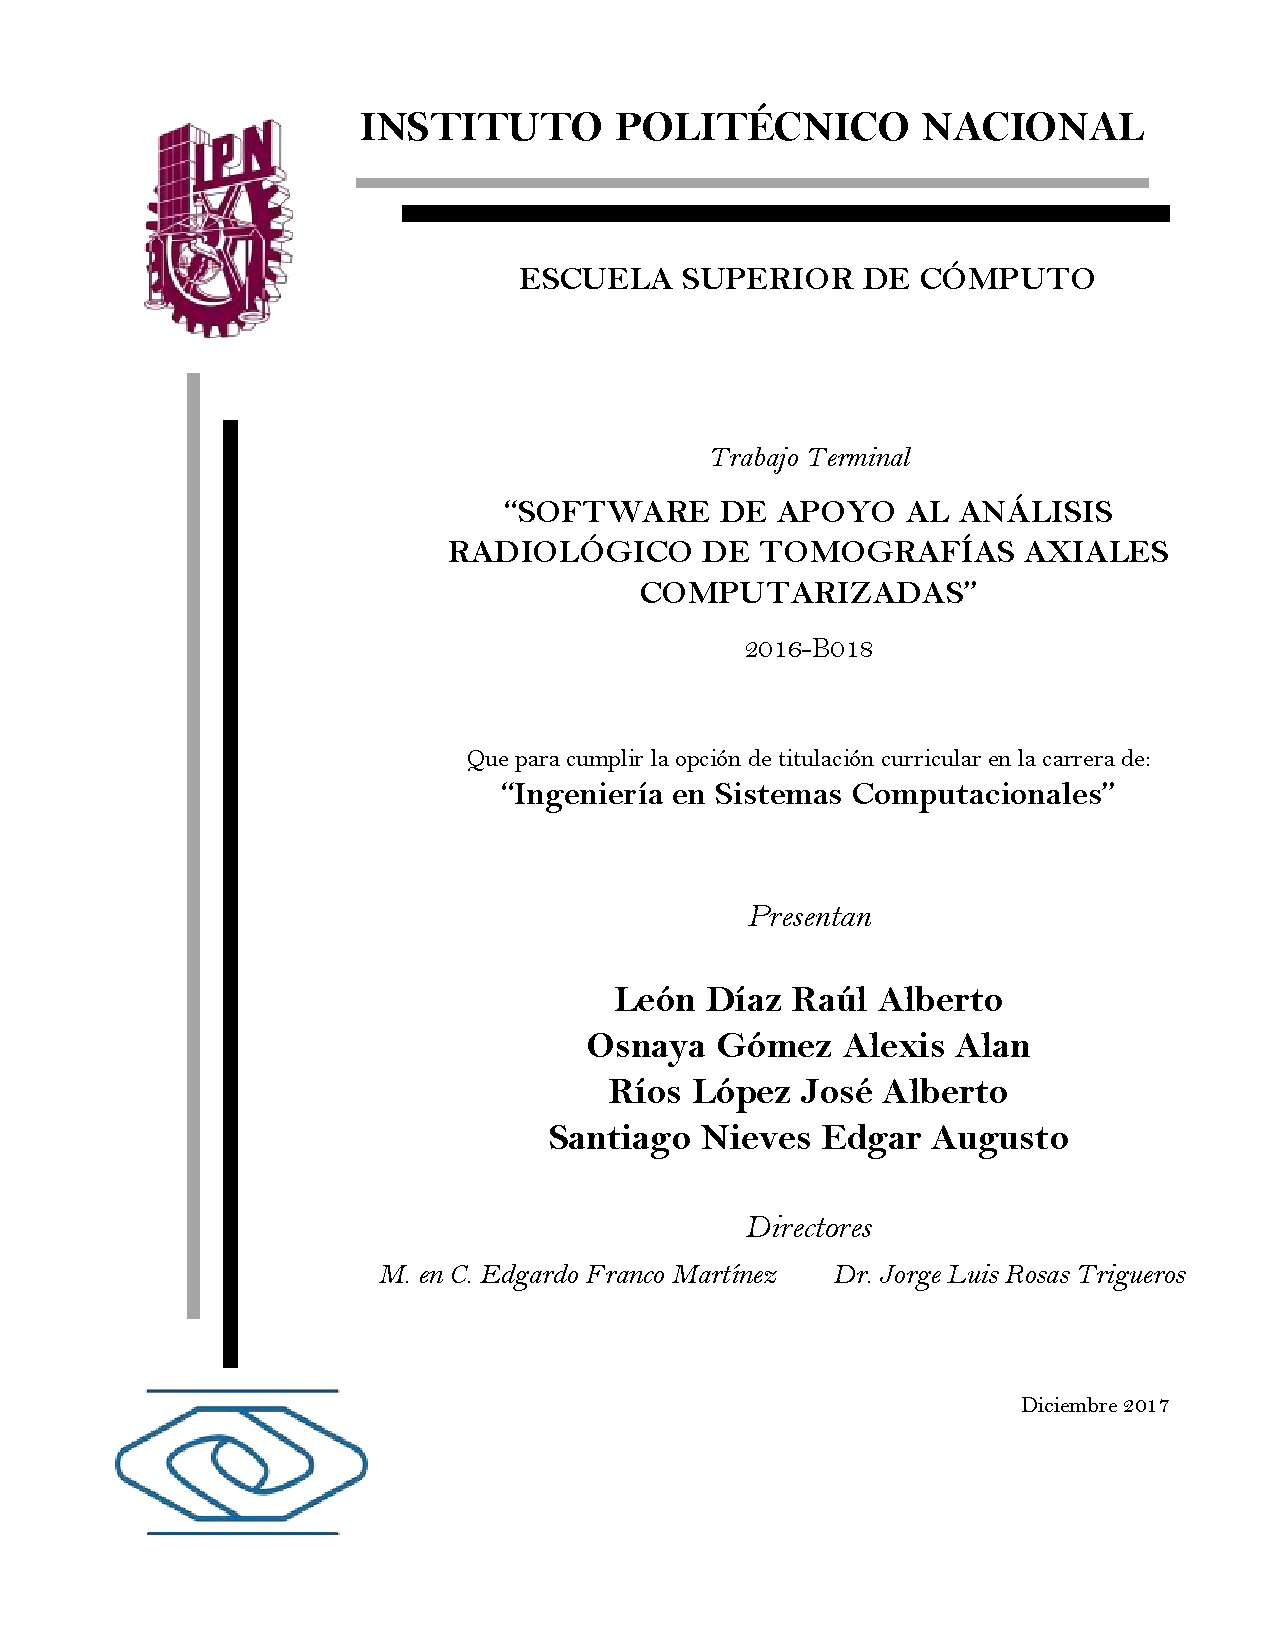
\includegraphics[scale=1]{portada.pdf}}} % pdf de fondo de portada
    \noindent
    \vspace{125mm}
\end{titlepage}
\endgroup

\tableofcontents

\cleardoublepage
\addcontentsline{toc}{chapter}{Lista de figuras} % para que aparezca en el indice de contenidos
\listoffigures % indice de figuras

\cleardoublepage
\addcontentsline{toc}{chapter}{Lista de tablas} % para que aparezca en el indice de contenidos
\listoftables % indice de tablas 

\chapter{Introducción}

\section{Antecedentes}
Los médicos consideran que la imagen médica ha sido y es, con mucha diferencia, el avance técnico que mayor impacto ha tenido en su práctica clínica.\\

El hombre(como otros mamíferos) es un animal esencialmente visual. Gran parte del cerebro humano está dedicado al procesamiento de la información visual; muchas estrategias mnemotécnicas y de aprendizaje rápido tratan de obtener ventaja de este hecho. Por esa razón, la información diagnóstica que proporcionan los sistemas de imagen es enormemente apreciada por el médico, hasta el punto de que, hoy en día, resulta difícil encontrar situaciones clínicas en las que no se haya hecho uso de una o más técnicas de imagen.\\ 

En 1895 se produce el descubrimiento que da lugar a la imagen médica como prueba diagnóstica cuya importancia no ha dejado de crecer hasta nuestros días: Wilhelm Rontgen, experimentando con descargas eléctricas en tubos de Crookes, observó que brillaba una placa de platinocianuro de bario al otro lado de la habitación, a pesar de estar el tubo encerrado en una caja de cartón. Además comprobó que esos ''misteriosos rayos''(bautizados por esta razón como rayos X) podían atravesar algunos objetos dejando su sombra en la pantalla.\cite{biom}\\ 

En el año de 1972 se publicó en la revista \textit{British Journal of Radiology} un artículo del ingeniero Sir Godfrey Newboold Hounsfield sobre una
técnica basada en rayos X, llamada tomografia computarizada, la cual hacía uso de métodos matemáticos desarrollados una decada antes por A. M. Cormack.
El nuevo método propuesto realizaba una división de la cabeza en varios cortes los cuales irradiaban a través de sus bordes, por lo cual la radiación emitida podía ser aislada dentro de la misma porción. La ventaja que este método presentaba frente a la técnica convencional de rayos X, era que la información no presentaba alteraciones debidas al material presente a los lados del corte en cuestión.\\ 

Con el fin de superar a la radiología convencional, el nuevo método pretendía superar 3 limitantes; la primera, la imposibilidad de mostrar toda la información de una escena tridimensional en una imagen radilógica bidimensional, debido a la superposición de los objetos en la imagen obtenida; la segunda limitante a vencer era la escaza capacidad de distinguir los tejidos blandos; finalmente, no era posible cuantificar las densidades que tenían los tejidos.\cite{TCFundamentos}  \\ 

El aumento de la utilización de la tecnología en la medicina buscó utilizar las computadoras para hacer diagnósticos automáticos con apoyo de las nuevas modalidades de imágenes médicas, sin embargo factores como la baja eficiencia de los equipos o la falta de accesibilidad a imágenes médicas no lo permitió. Posteriormente en los años 80's surgió un nuevo enfoque en el que se asumió que las salidas proporcionadas por la computadora podrían ser utilizadas por los radiólogos sin reemplazarlos, fue así como surgieron las herramientas de diagnóstico asistido por computadora o CAD(Computer-Aided diagnosis). En las CAD, los radiólogos utilizan la computadora para tener un ''segunda opinión'' sin embargo son ellos quienes toman la decisión final del diagnóstico.\cite{cad}\\

Con el surgimiento de la tomografía computarizada y otras modalidades de diagnóstico digital con imágenes usadas en las CAD, el ACR(American College of Radiology) y el NEMA(National Electrical Manufacturers Association) se dieron cuenta que se debía crear una forma en que dispositivos de diferentes fabricantes pudieran intercambiar información de las imágenes obtenidas. En 1993 surge DICOM(Digital Imaging and Communication in Medicine) como un estandar ante la problemática planteada.\cite{DICOMNEMA} DICOM no es sólo una imagen o formato de archivo, DICOM se encarga de cubrir la transferencia de información, almacenamiento y un protocolo de visualización construido y diseñado para satisfacer todas las necesidades de la medicina comtemporanea. Sin duda alguna DICOM es quien gobierna la práctica de la medicina digital.\cite{dicl}\\

La innovación tecnológica fue un parte aguas en la historia de la medicina y hoy en día es uno de los más importantes motores para el desarrollo de esta, permitiendo cada vez mejores y más rápidos diagnósticos de salud.

\section{Planteamiento del problema}
Hoy en día el diagnóstico asistido por computadora es usado principalmente en los métodos de diagnóstico que emplean contraste. Los métodos sin contraste, también llamados simples, no son comunmente asistidos por computadora después de haber realizado el estudio en el equipo médico especializado.\footnote{Información obtenida a través de una plática con Noé Hernandez, radiólogo en la Clínica de Médicina Familiar División del Norte.}\\

Los equipos necesarios para la generación de estudios como las TAC cuentan con herramientas de software muy potentes como el caso de SOMATOM por parte de la compañía SIEMENS o IQon Spectral de Philips, sin embargo los costos de las licencias así como de los equipos son muy elevados.\cite{guia}, \cite{guiad}\\

Las herramientas de asistencia que son accesibles en muchas ocasiones se limitan a algunas funciones básicas de análisis como rotar, escalar o hacer mediciones a las imágenes; algunas otras ofrecen más funciones como representación en 3D pero sólo es posible cuando las imágenes  cuentan más de un tipo de corte sobre el cuerpo humano.\cite{occi}, \cite{nifty}, \cite{osirix}, \cite{3dim}\\

\section{Propuesta de solución}
Para dar solución a la problemática anteriormente planteada se propone diseñar y desarrollar una herramienta de visualización y tratamiento de tomografías axiales computarizadas a partir de la información ofrecida por el archivo DICOM que las contiene, la cual permitirá a los especialistas una fácil y mejorada interpretación de  los resultados.\\

El primer paso será la decodificación de un archivo DICOM, una vez decodificada la imagen el usuario podrá observar la información contenida en el archivo DICOM mediante un visor. Adicionalmente, el usuario podrá utilizar diversas herramientas del sistema para que la información sea analizada y así obtener propiedades particulares de la imagen.

En la figura 1.1 se observa el diagrama general de funcionamiento del sistema.
\begin{figure}[H]
\centering
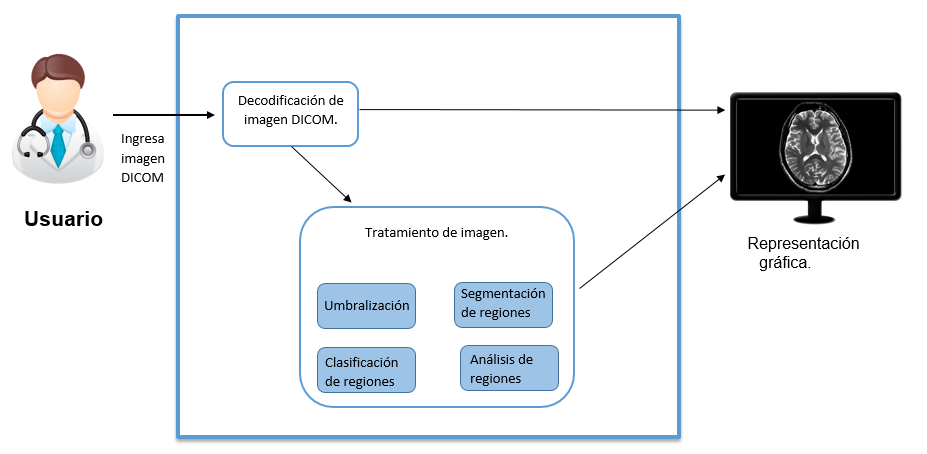
\includegraphics[width = 12 cm, height = 7 cm]{diagramageneral}
\caption{Diagrama del funcionamiento del sistema.}
Imagen de creación propia.
\end{figure}

\section{Justificación}
A lo largo de los años la evolución de la ciencia y la tecnología han permitido que el campo de la medicina se desarrolle y avance en un gran nivel, al permitir el desarrollo de medicinas y aparatos quirúrgicos que facilitan y minimizan el error dentro de los procesos, desafortunadamente no en todos los campos del área esto se ha logrado, cuando hablamos de errores médicos debemos tomar en cuenta que las consecuencias que estos pueden traer son muy delicadas pues en muchas ocasiones representan la vida o muerte de los pacientes.\\ 

“La interpretación de los estudios tomográficos radiológicos se realiza comúnmente con base a un análisis visual de las imágenes adquiridas de los equipos imageneológicos por parte del médico radiólogo, estos análisis son susceptibles a malas interpretaciones debido a error humano”, por esto es que decidimos realizar este trabajo con el fin de ayudar a la interpretación de estos estudios.\\

El uso de algoritmos computacionales para la delineación de estructuras anatómicas y otras regiones de interés del cuerpo humano se han vuelto muy importantes en la asistencia y realización de tareas radiológicas específicas. Estos algoritmos, llamados algoritmos de segmentación de imagen, tienen un papel muy importante en diversas aplicaciones de imágenes biomédicas , como la cuantificación del volumen de tejidos, diagnóstico, localización de patologías, estudio de estructuras anatómicas, planeación del tratamiento y cirugía computarizada.\cite{metodos}\\ 

Este trabajo terminal beneficia a la sociedad en general pues cualquiera puede necesitar un estudio por medio de una TAC y gracias al software propuesto se  podrá hacer un mejor análisis de la imagen.

\section{Objetivos}
\subsection{Objetivo General}
Desarrollar un software de asistencia al especialista para la interpretación adecuada de las tomografías axiales computarizadas.
\subsection{Objetivos Particulares}
\begin{itemize}
\item Leer e interpretar la información contenida en una imagen DICOM.
\item Umbralizar una imagen médica en formato DICOM.
\item Segmentar regiones determinadas dentro de una tomografía axial computarizada.
\item Clasificar regiones con base a distintos criterios.
\item Analizar distintas propiedades de regiones específicas.
\item Facilitar la interpretación de tomografías mediante un visor.
\item Proporcionar una visualización en 3D de las tomografías axiales computarizadas.
\end{itemize}


\chapter{Marco teórico}
En este capítulo se detallarán algunos terminos que ayudarán a una mayor comprensión del funcionamiento del sistema.
\section{Estado del arte}
La solución que se propone ante la problemática planteada no es una solución completamente nueva pues se han desarrollado anteriormente otros softwares que poseen una idea similar pero se atacan con un enfoque diferente. A continuación se listan algunos sistemas y trabajos similares a la propuesta realizada.

\hfill\break
\textbf{\textit{Image Analysis Software}}\cite{ims}
\\Algunas características ofrecidas por el software son las siguientes:
\begin{itemize}
\item Analiza modelos celulares complejos.
\item Gestiona eficazmente grandes cantidades de datos.
\item Visualiza modelos de células en 2D o 3D en tiempo real.
\item Muestra tejidos y cuantifica células.
\end{itemize}

\hfill\break
\textbf{\textit{3D-Doctor}}\cite{tridi}
\\El software proporciona las siguiente características:
\begin{itemize}
\item Puede leer imagenes DICOM, TIFF, BMP, JPEG, Interfile, PNG, PGM, GIF.
\item Contiene modelos 3D de exportación STL(ASCII y binario), 3D Studio(3DS)entre otros para la rápida creación de prototipos.
\item Mide área, superficie 3D, volumen 3D, distancia, perfil y región de un histograma.
\item Representación de diferentes tejidos.
\item Imagenes 3D CT/MRI pueden ser cortadas de nuevo facilmente a lo largo de un eje arbitrario.
\item Corte de imágenes para corregir las rebanadas de grosor desigual, el redimensionado de volumen y la rotación de imagen.
\end{itemize}

\hfill\break
\textbf{\textit{Análisis digital de imágenes tomográficas sin contraste para la busqueda de tumores cerebrales}}\cite{edgardo}
\\La tesis presentada nos ofrece estas características:
\begin{itemize}
\item Análisis digital de imágenes y reconocimiento de patrones para la busqueda de tumores cerebrales.
\item Codificación y extracción de la imagen a partir del archivo digital proporcionada por los sistemas PACS de la actualidad.
\end{itemize}


\hfill\break
\textbf{\textit{Reconstrucción tridimensional de estructuras internas del cuerpo humano a partir de tomografías axiales computarizadas}}\cite{titi}
\\Las características de este trabajo terminal desarrollado en la Escuela Superior de Cómputo se presentan a continuación:
\begin{itemize}
\item Sistema de reconstrucción tridimensional de estrucuturas internas del cuerpo humano mediante tomografías axiales computarizadas(TAC) en formato DICOM(''Digital Imaging and Communication in Medicine''). Dicho sistema proporciona una amplia manipulación del objeto generado en 3D.
\end{itemize}

\section{Imagen}
Una imagen puede ser definida como una función de dos dimensiones $f(x, y)$, donde $x$ y $y$ son coordenadas espaciales, y a la amplitud de la función $f$ en cualquier par de coordenadas $(x, y)$ se le llama \textit{intensidad} o \textit{niveles de grises} de la imagen en ese punto. Cuando $x$, $y$ y el valor de intensidad de la función $f$ son todos valores finitos y discretos, llamamos a la imagen una imagen digital. Notese que una imagen digital está compuesta de un número finito de elementos, cada uno de los cuales tiene una localización específica y un valor. Si cada posición de la imagen tiene una única medida, la imagen es llamada ''imagen escalar'', si las posiciones tienen más de una medida se les llama ''imágenes vectoriales'' o ''multicanal''. En las imágenes discretas en 2D la localización de cada medida es llamada ''pixel'' y en imagenes 3D se llama ''voxel'', en la figura 2.1 se observa la diferencia entre ambos terminos. \cite{metodos} \cite{imag}

\begin{figure}[H]
\centering

\includegraphics[width = 5 cm, height = 3 cm]{pixel}
\caption{Pixel y voxel.}
Imagen obtenida de \textit{https://carestreamdentalblogdotcom1.wordpress.com/2014/02/19/three-dimensional-basics-pixels-and-voxels/}
\end{figure}

\section{Imágenes médicas}
Una imagen médica es un conjunto de técnicas y procesos usados para crear imágenes del cuerpo humano, o partes de él, con propósitos clínicos  o para la ciencia médica.\\

Representa gráficamente una distribución espacial de una o más propiedades físicas o químicas del interior del cuerpo humano. Dos de los parámetros de mayor importancia son el contraste y la resolución. \\

El contraste se define como la diferencia en la intensidad entre un punto de  la imagen y determina lo que podemos ver en ella, en el caso del contraste en una imagen médica es muy importante tener el conocimiento de diversos parámetros físicos o químicos que ayuden a entender lo que está siendo representado.\\

La resolución por su parte se define como la nitidez con la que se percibe una imagen observada por un instrumento óptico. Nos ayuda a encontrar todas las características de la imagen para así distinguir y analizar detalles.\cite{essen}\\ \\
Modalidades de las imágenes médicas.\cite{modim}\\
\begin{itemize}
\item Radiología: Es el uso médico de la radiación para diagnosticar y tratar diversos problemas de salud. A partir de la utilización de rayos gamma, rayos X y otras clases de rayos, es posible obtener imágenes internas del organismo.
\item Medicina nuclear: Es una especialidad médica que realiza diagnósticos y tratamientos mediante la utilización de trazadores o radiofármacos. Realiza estudios de órganos y sistemas desde el punto de vista funcional.  La Medicina Nuclear se diferencia de las otras técnicas de imagen en que realiza estudios fisiopatológicos. Es decir da una visión de cómo funciona el organismo.
\item Ecografía: Utiliza ondas sonoras de alta frecuencia para observar órganos y estructuras al interior del cuerpo.
\item Resonancia magnética: Se considera como una técnica no invasiva, ya que no requiere la introducción de herramientas o elementos en el cuerpo ni tiene consecuencias para el paciente. La información que se obtiene a través de la resonancia magnética es convertida en imágenes en una computadora, permitiendo que el profesional observe, de este modo, el interior del organismo.
\item Endoscopia: Es un procedimiento que permite que el médico vea el interior del cuerpo. Utiliza un instrumento llamado endoscopio o tubo visor. Los endoscopios tienen una cámara diminuta unida a un tubo largo y delgado.
\end{itemize}

\section{Tomografía computarizada}
El descubrimiento y el desarrollo de la TC (Tomografía Computarizada) revolucionó el diagnóstico por imagen en medicina. La TC es una técnica digital y matemática de diagnóstico por imagen, que origina cortes tomográficos en los que cada capa no está contaminada por estructuras borrosas procedentes de la anatomía adyacente. Lo más importante, la TC permite la diferenciación y cuantificación de los tejidos duros y blandos. De este modo, por primera vez en las técnicas de imagen en medicina, el radiólogo podía visualizar los tejidos duros y blandos sobre una imagen, sin llevar a cabo un procedimiento invasivo sobre el paciente, como puede ser la inyección de medios de contraste.\\
La TC produce imágenes axiales de la anotomía de un paciente. Dichas imágenes se obtienen de forma perpendicular al eje mayor del cuerpo como se muestra en la figura 2.2.

\begin{figure}[H]
\centering
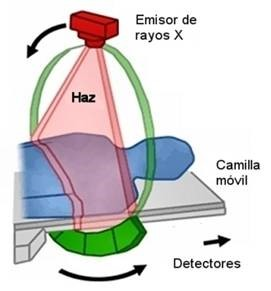
\includegraphics[width = 5 cm, height = 5 cm]{tac}
\caption{Cortes axiales en TAC.}
\end{figure}

La TC es una técnica de diagnóstico para imagen digital. La fuente de rayo X se une rígidamente a un dispositivo detector de la geometría en abanico de los rayos, que rota 360 grados alrededor del paciente y recoge los datos. El detector de imagen presenta un estado gaseoso o sólido, lo que produce señales que sirven como datos de entrada para un ordenador exclusivo. Dicho ordenador procesa los datos mediante técnicas de retroproyección con algoritmo de Fourier, desarrolladas por primera vez por Hounsfield para dar lugar a imágenes de TC. Las imágenes de TC son en sí mismas tridimensionales, de 512 X 512 pixeles típicamente, con un espesor definido por la separación de cortes de la técnica de imagen. Cada elemento de la imagen de TC se denomina vóxel, el cual presenta un valor, al cual se le refiere en unidades de Hounsfield, que describe la densidad de la imagen de TC en dicho punto.\cite{prote}\\
 
El resultado final de la reconstrucción por la computadora, es una matriz de números, que no es conveniente para su visualización en pantalla, por lo que un procesador se encarga de asignar a cada número o rango de números, un tono gris adecuado. Los valores numéricos de la imagen de tomografía computada, están relacionados con los coeficientes de atenuación, debido a que la disminución que sufre el haz de rayos X, al atravesar un objeto, depende de los coeficientes de atenuación lineales locales del objeto.\cite{tacuro}\\

Algunas ventajas que ofrece esta técnica es el tiempo de exploración del orden de segundos en las modernas generaciones de aparatos, unido a su baja inocuidad (capacidad de hacer daño), lo que permite repetirlo cuantas veces sea necesario, así como su alta fiabilidad diagnóstica de certeza media, que alcanza el 85\%, superando con creces los resultados de todas las técnicas exploratorias clásicas juntas, aunque, justo es decirlo, no las desplaza en absoluto, sino que todas ellas se complementan mutuamente.\cite{tcraneo}\\

Los posibles usos de este método diagnóstico, son los siguientes: anormalidades del cerebro y medula espinal, tumores cerebrales y accidentes cerebro vasculares, sinusitis, aneurisma de aorta, infecciones torácicas, enfermedades de órganos como el hígado, los riñones y los nódulos linfáticos del abdomen y muchos otros más.\cite{tacuro}\\

\section{DICOM}
DICOM (Digital Imaging and Comunications in Medicine) es un estándar propuesto y administrado por la National Electrical Manufacturers Association (NEMA) en 1992. Especifica mecanismos de codificación, almacenamiento y transmisión de imágenes médicas; para llevar a cabo un análisis digital de imágenes médicas, generalmente se utilizan visores DICOM que implementan el estándar ya que con ellos es posible visualizar y exportar las imágenes a formatos de imagen digital comunes (JPG, PNG, BMP, etc.). \cite{dicdie}
El formato genérico del archivo de DICOM consiste en dos partes diferenciadas:
\begin{enumerate}
\item Una cabecera (header) con multitud de campos estandarizados que especifican datos administrativos (datos del paciente, hospital donde se realizó, entre otros), datos sobre el estudio y la sintaxis de transferencia UID  que específica la codificación y la compresión del conjunto de datos que le sigue.
\item Un conjunto de datos (data set) de DICOM, que contiene la imagen o las imágenes especificadas que pueden estar comprimidas con distintos estándares, en la figura 2.3 se muestra la estructura básica de un archivo DICOM.
\end{enumerate}

\begin{figure}[H]
\centering
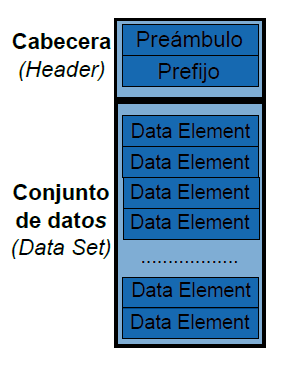
\includegraphics[width = 7 cm, height = 8 cm]{estructura}
\caption{Estructura de un archivo DICOM}
\end{figure}

\section{Escala de Hounsfield}
El elemento individual de la imagen de TC es el vóxel, que tiene el valor, referido en unidades de Hounsfield, que describe la densidad de la imagen de TC en ese punto. Cada vóxel contiene 12 bits de datos y va desde -1000(aire) hasta las +1000 de unidades Hounsfield. Los escáneres de TC tienen un valor estandarizado de Hounsfield de 0 para el agua. La escala de densidad de los TC es cuantitativa y significativa en cuanto a la identificación y diferenciación de las estructuras y los tejidos.\cite{hounsuno}\\

La escala de Hounsfield (HU) es una transformación lineal de la medida original del coeficiente de atenuación, basada en la radiodensidad del agua destilada, establecido en el STP (Estándar presión y temperatura) y se define como igual a 0HU, mientras que la radiodensidad del aire en STP se define como -1000HU; lo anterior proporciona al tejido óseo más denso (hueso compacto) valores cercanos a +1000HU. La figura 2.4 muestra los valores aproximados para algunos tejidos y órganos comúnmente estudiados.\\

La escala Hounsfield se extiende a lo largo de 2000 unidades que difícilmente serían distinguibles si se le asignara a cada unidad un nivel de brillo distinto en un monitor de vídeo, esto debido a que el ojo humano no es capaz de distinguir más de 40 tonalidades de brillo diferentes, representar en una imagen toda la gama de valores de la escala de Hounsfield conlleva a no poder visualizar una gran cantidad de información. Por lo tanto, solo se representa mediante una escala de grises un sector parcial de los valores de la TC con el fin de solo visualizar el órgano o tejido estudiado y su detalle.\cite{hounsdos}\\
\begin{figure}[H]
\centering
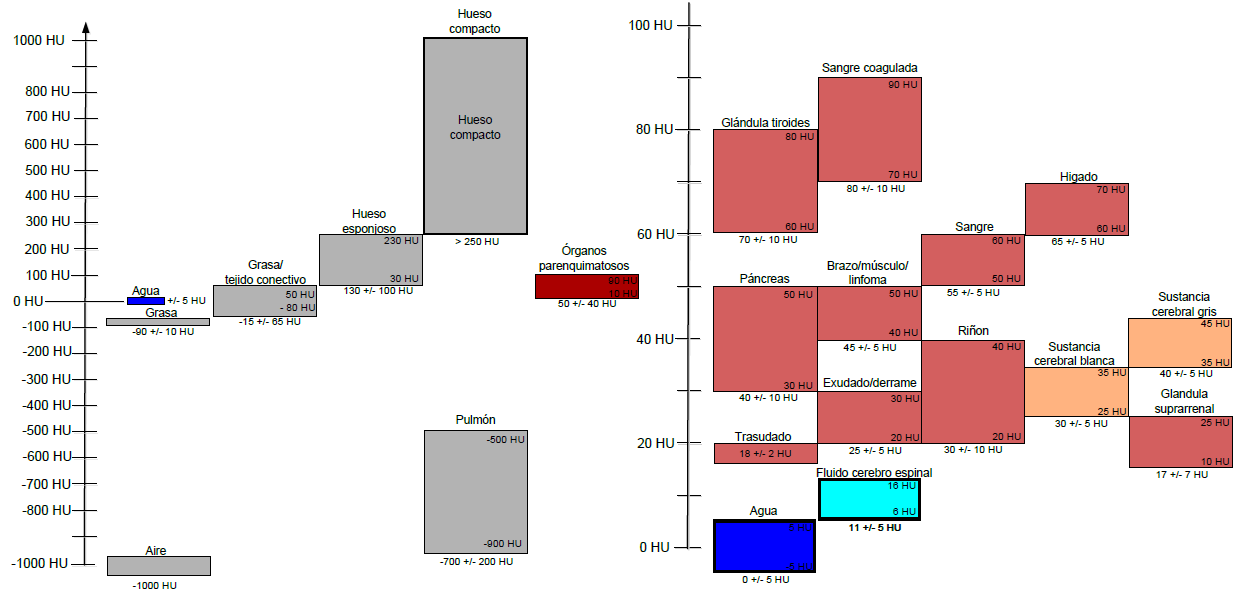
\includegraphics[width = 13 cm, height = 10 cm]{escala}
\caption{Escala de Hounsfield}
\end{figure}



\section{Segmentación}
La segmentación de imágenes está definida como el particionado de una imagen en regiones constituyentes que no se solapan y las cuales son homogeneas con respecto a alguna característica como intensidad o textura. Si el dominio de la imagen está dado por $\Omega$, el problema de la segmentación es determinar cuales conjuntos $S_{k} \subset \Omega$, cuya unión, es el dominio $\Omega$ completo. Así, los conjuntos que componen una segmentación deben satisfacer \begin{equation} \Omega = \bigcup_{k = 1}^{K} S_{k} \end{equation}
donde $S_{k} \bigcap S_{j} = \o$ para $ k \neq j$ y cada $S_{k}$ está conectado. En un funcionamiento ideal, los métodos de segmentación encuentran aquellos conjuntos que corresponden a distintas estructuras anatómicas o regiones de interés en la imagen.\\

Si no tomamos en cuenta la restricción que indica que las regiones estén conectadas el proceso de determinar los conjuntos $S_{k}$ es llamado ''clasificación de pixeles'', y los conjuntos se llaman ''clases''. La clasificación de pixeles es una meta deseable en las imagenes médicas, especialmente cuando regiones desconectadas que pertenecen a la misma clase de tejido deben ser identificadas. Determinar el número total  de clases \textit{K} en la clasificación de pixeles puede ser un gran problema. A menudo, suponemos que el valor de \textit{K} se conoce con base al conocimiento previo de la anatomía considerada. Por ejemplo, en la segmentación de una imagen cerebral obtenida a partir de una resonancia magnética, es común asumir que \textit{K} = 3, correspondiente a las clases de los tejidos de materia gris, materia blanca y el fluido cerebroespinal.\\

El etiquetado es el proceso de asignar un significado importante a cada región o clase, este procedimiento se puede llevar a cabo como un proceso separado de la segmentación. En este proceso se mapea el índice numérico \textit{k} del conjunto $S_{k}$ a una denominación anatómica. En la imagenología médica, las etiquetas por lo general son visualmente detectables con obviedad y pueden ser determinadas en una revisión por un físico o un técnico. El etiquetado automatizado por computadora es deeseable cuando las etiquetas no son obvias y en sistemas con procesos automatizados. Una típica situación que involucra etiquetado sucede en las mastografías digitales, en la cual la imagen es segmentada en diferentes regiones, las cuales después son clasificadas como sanas o tejido con tumor.\cite{metodos}

\subsection{Umbralización}
Las ténicas de umbralización segmentan imágenes escalares al generar una partición binaria a través de las intensidades de la imagen. La figura \textit{2.5a} muestra el histograma de una imagen escalar que aparentemente posee 3 clases, correspondientes a las 3 modas. El procedimiento de umbralización trata de determinar un valor de intensidad, llamado ''umbral'', el cual separa las clases deseadas. Logramos la segmentación cuando agrupamos los pixeles con intensidades mayores a las del umbral en una clase y todos los otros en otra clase. Dos umbrales potenciales se observan en la figura \textit{2.5a} en el valle del histograma. Determinar más de un valor umbral es un proceso llamado multiumbralización.\\

\begin{figure}[H]
\centering
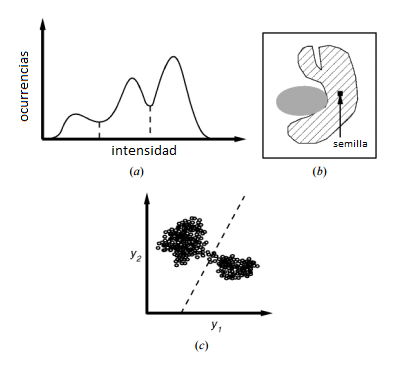
\includegraphics[width = 10 cm, height = 10 cm]{umbral}
\caption{Métodos de características espaciales y región creciente. (a)Histograma con 3 aparentes clases. (b)Característica espacial en 2-D. (c)Ejemplo de región creciente.}
\end{figure}

La umbralización es un procedimiento simple pero efectivo para segementar imágenes en las cuales diferentes estructuras tienen intensidades contrastantes u otras características cuantificables. A menudo la partición de la imagen se genera en interacción con el usuario aunque también existen métodos automatizados.\\

La umbralización a menudo es utilizada como la primera de las operaciones en una secuencia de procesamiento de imagenes. Se ha aplicado en mastografías digitales, en las cuales usualmente hay presentes dos clases de tejidos --sanos y con tumores. Su principal limitación, es que en su forma más simple, sólo se generan dos clases y no se puede aplicar a imágenes multicanales. Además, la umbralización comunmente no toma en cuenta las características espaciales de la imagen. Esto causa que sea sensible a las inhomogeneidades de ruido e intensidad, lo cual puede pasar en la resonancia magnética. Ambos sucesos corrompen de manera significante el histograma de la imagen haciendo más difícil la separación. Por estas razones, se han propuesto variaciones a la umbralización clásica aplicada en imágenes médicas basadas en intensidades y conectividad. \cite{metodos}

\subsection{Región creciente}
El método de región creciente es una técnica para extraer una región de la imagen que esta conectada basada en un criterio predefinido. Este criterio puede estar basado en la intensidad y/o bordes de la imagen. En su forma más simple, la región creciente requiere una semilla que es seleccionada manulamente por el operador y extrae todos los pixeles conectados a la semilla inicial basado en un criterio predefinido.\\

Por ejemplo, un posible criterio puede ser hacer crecer una región hasta que se tope con el borde de la imagen.\\

Esto es representado en la figura 2.5b, en el cual una región creciente ha sido usada para aislar una de las estructuras.\\

Como la umbralización, la región creciente raramente es usada por si sola, generalmente es usada dentro de un conjunto de operaciones de procesamiento de imagen, particularmente para la delineación de pequeñas estructuras como tumores o lesiones. La principal desventaja de la región creciente es que requiere una interacción manual para obtener la semilla. Aparte, para cada región que necesita extraerse, una semilla debe plantarse. El algoritmo Split-Merge (dividir y juntar) está relacionado con región creciente.\\

La región creciente puede ser sensible al ruido, causando asi que las regiones extraidas puedan tener hoyos o incluso puedan ir desconectadas. De forma inversa, los efectos de volumen parcial pueden lograr que regiones separadas se conecten entre si. Para ayudar a resolver estos problemas, se propuso un algoritmo homotópico de región creciente, para preservar la topología entre una región inicial y una región extraída.

\textit{Split and Merge.}
Las técnicas de Split and Merge intentan solucionar los problemas de ruido y los falsos bordes usando una medidad controlada de homogeneidad.
El objetivo es segmentar automaticamente la imagen en un mínimo número de regiones que intentan representar areas de uniformidad, produciendo bordes con características relacionadas con la resolución de la imagen. La alternativa aproximada de región creciente inicia con un valor de semilla e intenta encontrar la extensión de una región local que obedece al criterio de homogeneidad dado por la semilla.\\
Normalmente el algoritmo comienza con la hipótesis de que la imagen completa es una única región, entonces analiza la homogeneidad de la misma (mediante un cierto criterio y propiedades). Si existe homogeneidad, la imagen se encuentra ya segmentada, si no es así, entonces la región es dividida en 4 regiones.
Este proceso se repite para cada una de las regiones generadas hasta que el proceso de división no puede llevarse a cabo.\\
Una vez que se ha llevado a cabo el proceso de división, se comprueba para cada región generada, si es posible unirla con una región adayacente (lógicamente si satisfacen el criterio de homogeneidad establecido). El proceso termina cuando no se pueden fusionar más regiones.\cite{split}

\begin{figure}[H]
\centering
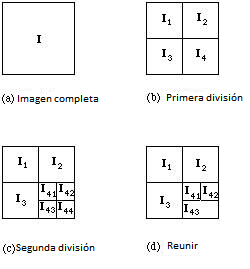
\includegraphics[width = 7 cm, height = 7 cm]{split}
\caption{Ejemplo iteración algoritmo Split and Merge.}
\end{figure}


\subsection{Clasificadores}
Los métodos clasificadores son técnicas de reconocimiento de patrones que buscan una partición a una característica espacial dada por un una imagen usando datos con etiquetas conocidas.
Una característica espacial es un rango de espacio de cualquier función de una imagen, siendo la característica espacial más común las intensidades de la imagen. Un histrograma, como se muestra en la figura 3a, es un ejemplo de una característica espacial de una dimensión. La figura 3c muestra un ejemplo de una característica espacial en 2-d con aparentemente dos clases.
Así como una figura espacial pudo haberse sido generada de un eco dual de una resonancia magnética, en la cual un eje representa las intensidades de un protón de una imagen densamente ponderada y otro eje representa las intensidades de la ponderación T2 de la imagen.
Todos los pixeles con sus características asociadas son agrupadas en una clase en el lado izquierdo de la partición.
Los clasificadores son conocidos como métodos supervisados ya que requieren de datos entrenados que son segmentados manualmente y se usan como referencia para segmentar automaticamente nuevos datos.
Hay muchas maneras en la cual los datos entrenados puedan ser aplicados a métodos clasificadores. Un clasificador simple es el clasificador de vecino más cercano, en el cual cada pixel es clasificado en la misma clase donde estan los datos entrenados con la intensidad más cercana. El clasificador del k-ésimo vecino mas cercano es considerado un clasificador no paramétrico porque no hace supociciones subyacentes sobre la estadística de la estructura de los datos.
Otro clasificador no parametrico es la ventana de Parzen, en  la cual la clasificación está hecha por un proceso de decisión ponderada dentro de una ventana predefinida de característica espacial, centrado en la intensidad de pixeles no etiquetados.

Un clasificador usado comunmente es el de  máxima similitud o clasificador Bayes. Este asume que la intensidad de los pixeles son muestras independientes de una mezcla de distribución de probabilidad, usualmente Gaussiana. Este mezcla, es llamada modelo de mezcla finita y esta dada por la siguiente función de probabilidad:

\begin{equation} f(y_{j};\theta,\pi) = \sum_{k = 1}^{K} \pi_{k} f_{k} (y_{j} ; \theta_{k}) \end{equation}


donde $y_{j}$ es la intensidad del pixel $j$ , $f_{k}$ es el componente de probabilidad de la función de densidad parametrizada por $\theta_{k}$, y $\theta = [\theta_{1},...,\theta_{k}]$. Las variables $\pi_{k}$ son coeficientes mezclados donde miden la contribución para cada densidad de la función y $\pi = [\pi_{1},...,\pi_{k}]$.
Los datos entrenados son recolectados a traves de obtener muestras reprensentativas de cada componente del modelo mezclado y el estimado para cada theta.

Para mezclas Gaussianas, esto significa un estimado de K-medias, covarianzas y coeficientes mezclados.
La clasificación de los nuevos datos es obtenida asignando cada pixel a la clase con la más alta probabilidad posterior. Cuando los datos en verdad siguen una mezcla finita Gaussiana, el clasificador de  máxima similitud puede realizarse de forma correcta y es capaz de proveer una segmentación suave compuesta por probabilidades posteriores.

Los clasificadores estandar requieren que las estructuras que van a ser segmentadas posean características cuantificables distintas. Como los datos entrenados pueden etiquetarse, los clasificadores pueden transferir estas estiquetas a nuevos datos siempre y cuando su característica espacial se distinga lo suficiente en cada etiqueta.
Siendo notorio, los clasificadores son relativamente computacionalmente eficientes, no como los métodos de umbralización que pueden ser aplicados para imágenes multicanal. Una desventaja de los clasificadores es que por lo general no realizan ningún modelado espacial. Otra desventaja es que requieren una interacción manual para obtener los datos de entrenamiento.
Se pueden adquirir conjuntos de entrenamiento para cada imagen que requiere ser segmentada, pero esto puede consumir mucho tiempo y puede ser laboriosos. Por el otro lado, usar un conjunto datos de entrenamiento para un gran número de escaneo de numeros puede llevar a resultados parciales que no toman en cuenta la variedad anatómica y fisiológica entre diferentes sujetos.\cite{metodos}

\subsection{Clustering}
Los algoritmos de clustering escenciamente realizan la misma función de los métodos clasificadores pero sin usar datos entrenados. Aparte, son metodos no supervisados. Para compensar la falta de datos entrenados, los métodos de clustering iteran alternadamente entre imagenes segmentada y caracterízan las propiedades de cada clase. En cierto sentido, los métodos de clustering se entrenan a si mismos usando los datos disponibles.
Los tres algoritmos de clustering mas comunes son el K-means o ISODATA algorithm, el fuzzy c-means algorithm y el expectation-maximization algorithm.\cite{split}

\subsubsection{Algoritmos de clustering}
\begin{enumerate}[A.]
\item \textit{Algoritmo K-medias.} En el clustering de K-medias, particiona una coleccion de datos en k números de grupos de datos. Clasifica un conjunto de datos ya dados en k números de cluster desarticulados. El algoritmo de K-medias es separarado dos fases.
En la primer fase se calcula el centro k y en la segunda fase se traslada cada punto al cluster en el cual tiene el centro mas cercano desde su respectivo punto de dato. Hay diferentes métodos que definen la distancia entre el centro más cercano y uno de los métodos mas utilizados es la distancia Euclidiana. Una vez que el agrupamiento ya se realizó se recalcula un nuevo centro para cada cluster y basado en ese centro, una nueva distancia Euclidiana es calculada entre cada centro y cada punto y asigna los puntos al cluster que tiene la mínima distancia Euclidiana.
Cada cluster en la partición es definido por sus objetos miembros y por su centro. El centro de cada cluster es el punto en el cual la suma de distancias de todos los objetos en el cluster es minimizada. Por lo tanto K-medias es un algoritmo iterativo en el cual se minimiza la suma de las distancias de cada objeto hacia el centro del cluster.\cite{kmed}

\item \textit{Algoritmo Fuzzy C-Media.} Itera entre las probabilidades posteriores y calcula la máxima probabilidad estimada de la media, covarianzas y coeficientes mezclado de un modelo mixto.

\item \textit{Algoritmo EM.} EM es uno de los algoritmos más comunmente usados para la estimación de densidad en puntos de datos en una configuración sin supervisar. El algoritmo depende en encontrar estimaciones de máxima verosimilitud de los parámetros cuando un modelo de dato depende de ciertas variables latentes. En el algoritmo EM, se realizan alternaciones en los pasos de expectación y maximización iterativamente hasta que el resultado converga. El paso de E calcula una expectación de una verosimilitud incluyendo las variables latentes como si fueran observadas, y el paso de maximización  calcula la máxima verosimilitud estimada por los parámetros maximizando la verosimilitud esperada encontrada en el paso E. Los parametros encontrados en el paso de maximizacion son usados despues por otro paso E y el proceso se repite hasta que converja.\cite{em}

\end{enumerate}

\chapter{Análisis}
\section{Comparación de software}
En esta sección se analizan algunas características que se considerarán para el desarrollo del sistema, estas características son el sistema operativo y los lenguajes de programación, esto con el fin de elegir las herramientas que puedan ser más útiles para la construcción del sistema.

\subsection{Sistemas operativos}
La elección del sistema operativo es primordial para el desarrollo de un sistema ya que con base a este se pueden encontrar librerías específicas para el desarrollo del mismo. En la tabla 3.1  se hace una comparación entre dos sistemas operativos detallando algunas características que se considerarán para el desarrollo del sistema.

\begin{table}[H]
\begin{center}
\begin{tabular}{|p{25mm}|p{60mm}|p{60mm}|}
\hline
Sistema operativo & Ventajas & Desventajas\\
\hline \hline 
Linux & Es un sistema operativo de software libre. Cuenta con una gran estabilidad. Seguridad porque es un sistema operacional diseñado con la idea de Cliente-Servidor con permisos de acceso y ejecución a cada usuario. Las vulnerabilidades son detectadas y corregidas más rápidamente que cualquier otro sistema operativo.\cite{so} & A pesar de ser un sistema operativo de software libre hay muchas aplicaciones que no corren en Linux. Linux no cuenta con una empresa que lo respalde por lo que no cuenta con soporte concreto. La configuración no es tan trivial.  Tiene una gran cantidad de distribuciones.\cite{so}\\
\hline
Windows & Es el sistema operativo más conocido en el mundo por lo que cuenta con gran cantidad de aplicaciones. Interfaz gráfica amigable. Cuenta con muchos asistentes de configuración. La mayoría de los médicos están más familiarizados con Windows.\cite{so} & Cuenta con más brecha de seguridad ya que muchos virus están hechos para este sistema operativo. Costo elevado. Usuario no tiene acceso al código. Baja estabilidad.\cite{so}\\
\hline
Mac OS & Interfaz intuitiva. Su vulnerabilidad ante malware es muy baja.  Gran rendimiento.\cite{mac} & El hardware es caro. No existe una gran cantidad de software para Mac. La mayoría de los accesorios deben ser de la misma compañía.\cite{mac}\\
\hline
\end{tabular}
\caption{Tabla comparativa de sistemas operativos.}
\end{center}
\end{table}

\subsection{Lenguajes de programación}
Para el desarrollo del sistema se deben de tomar en cuenta las características que te brindan algunos lenguajes de programación, ya que todos los lenguajes tienen sus ventajas así como sus desventajas. A continuación en la tabla 3.2 se listan tres lenguajes de programación junto con sus ventajas y desventajas.

\begin{table}[H]
\begin{center}
\begin{tabular}{|p{25mm}|p{60mm}|p{60mm}|}
\hline
Lenguaje de programación & Ventajas & Desventajas\\
\hline \hline 
Java & El compilador del lenguaje de Java  restringe ciertas operaciones para corregir errores. Estandariza muchas estructuras y operaciones como listas, manejo de conexiones de interconexiones (network connections) y provee interfaces gráficas de usuario(graphical user interfaces). Es orientado a objetos. Manejo automático de la memoria.\cite{java} & Al tener que ser ejecutado mediante una maquina virtual (JVM) hace que no sea tan rápido como  otras tecnologías, un ejemplo C++.\cite{java}\\
\hline
C++ & Usa múltiples paradigmas de programación (POO, estructurado). Puede compilar y ejecutar código en C. Provee un desempeño y manejo de memoria eficiente. Alto nivel de abstracción.\cite{cplus} & Uso de DLLs (librerías dinámicas) muy complejos. No tiene un recolector de basura. No es seguro porque tiene apuntadores, funciones amigas y variables globales.\cite{cplus}\\
\hline
Python & Lenguaje de programación multi-paradigma, permite varios estilos de programación: orientado a objetos, estructural y funcional.
Gran soporte e integración con otros lenguajes y herramientas.
Lenguaje estable, confiable y fácil de aprender.
Te permite realizar aplicaciones con menos código que con otros lenguajes. Cuenta con una gran cantidad de Framewoks que se pueden utilizar.\cite{vibora}
 & Ya que es un lenguaje interpretado es lento. No es la mejor opción para el manejo de memoria.\cite{vibora}\\
\hline
C\# & Declaraciones en el espacio de nombres. Tipos de datos: Existe un rango más amplio y definido de tipos de datos que los que se encuentran en C, C++ o Java. Atributos: Cada miembro de una clase tiene un atributo de acceso del tipo público, protegido, interno, interno protegido y privado. Pase de parámetros: Se puede declarar los métodos para que acepten un número variable de parámetros. & Se tiene que conseguir una versión reciente de Visual Studio .NET. Se tiene que tener algunos requerimientos mínimos del sistema para poder trabajar adecuadamente como contar con Windows NT 4 o superior. Se requiere mucho espacio de almacenamiento para su instalación. \cite{sisharp}
\end{tabular}
\caption{Tabla comparativa de lenguajes de programación.}
\end{center}
\end{table}

\subsection{Elección de librerías}
El uso de librerías facilitan el desarrollo del sistema ya que hay mucho código que se puede utilizar. En este sección se describen las librerías que se van a implementar.

\subsubsection{Descripción general de PYDICOM}
PYDICOM es un paquete puro de python para trabajar con archivos DICOM tales como imágenes médicas, reportes y objetos de radioterapia. PYDICOM facilita leer estos archivos complejos en estructuras naturales de lenguaje python para su fácil manipulación. Se modifica su dataset que puede ser escrito de nuevo en un formato de archivo DICOM. PYDICOM no se trata de solo ver las imágenes, esta diseñado para manipular elementos de datos en archivos DICOM con código python. Además es fácil de instalar y usar, y ya que es un paquete de python, debe correr en cualquier lugar donde corre un programa en python.
Una limitación presente en esta librería es que los datos comprimidos de píxeles (por ejemplo JPEG) no se pueden alterar de una manera inteligente como es posible con los pixeles que no se encuentran comprimidos. PYDICOM tiene una licencia basada en la licencia de MIT. La librería pydicom es soportada por\\ varios sistemas operativos tales como: Linux, Mac OS, Windows.\cite{pydi}\\

Dataset es el objeto base en el modelo de objetos de pydicom. Es el objeto principal con el cual se trabajará directamente. Dataset es un derivado del \textit{dict de python} (diccionario de python), así que este hereda los métodos de dict. En otras palabras es una colección de la paridad llave:valor, donde la llave es la etiqueta DICOM y el valor es una instancia del elemento de datos.\cite{pydi}

PYDICOM no es una librería exigente, los únicos requisitos para utilizarla son:
\begin{itemize}
\item Tener una versión de compilador mayor a la 2.4.
\item Tener la librería NumPy para la manipulación de los datos de los pixeles.
\end{itemize}

\subsubsection{Descripción general de DCM4CHE}
DCM4CHE es un conjunto de aplicaciones  utilizadas mundialmente por profesionales de la salud, proyectos de investigación , aplicaciones de software libre y software comercial. DCM4CHE es una implementación de software libre de alto rendimiento del estandar DICOM. Está desarrollado en el lenguaje de programación Java. Esta herramiento es un sistema JEE(Java Enterprise Edition) y JMX(Java Management Extensions) que se despliega dentro del servidor de aplicaciones JBoss para proveer diversos servicios clínicos. Se puede usar para diversos propósitos, los más populares son:
\begin{enumerate}
\item Manejo y almacenamiento de archivos DICOM.
\item PACS(Sistema de archivo y transmisión de imágenes) cuando se usa con un visor.
\end{enumerate}
En un principio DCM4CHE fue diseñado con la intención de ser utilizado por Sun como un JSR(Java Specification Request) para cualquier aplicacion de DICOM en Java. Con eso en mente, la herramienta fue separada en una aplicación de interfaz y otra de aplicación.\cite{dcm}\\
Algunas de las características más importantes son:
\begin{itemize}
\item Provee una interfaz de usuario basada en la web.
\item Permite un manejo de objetos DICOM a través de la conversión a estándares del sistema. 
\item Uso del servidor HL7.
\item Acceso web a diversas fuentes de información. 
\item Exportación a CD.
\end{itemize}

\section{Elección de herramientas para el desarrollo}
Con base a lo expuesto anteriormente en esta sección se hace la selección de las herramientas a utilizar para el desarrollo del sistema.\\
\subsection{Software}
\textbf{Lenguajes}
\textit{Python}
No es un secreto que Python es uno de los lenguajes de programación más populares, durante los últimos 5 años, Python se ha sostenido como el lenguaje de programación número uno. Python es uno de los favortios entre los desarrolladores debido al énfasis que pone en su legibilidad y su eficiencia, especialmente cuando se comprara con otros lenguajes como Java, PHP o C++. Python permite crear más funciones en una menor cantidad de líneas de código. Python es rápido de aprender para cualquiera.\\
La belleza de Python -además de su simplicidad- se basa en las reglas de programación sobre las cuales está creado el lenguaje. Algunos de estos principios son:
\begin{itemize}
\item La legibilidad es muy importante.
\item Menos es más.
\item Lo complejo está bien, pero no complicado.
\item Lo claro es mejor que lo implícito.
\end{itemize}

\textit{Justificación.}\\ Se escogió este lenguaje debido a las librerías con las que cuenta además del posible manejo de la información que permite, además la sencillez que este lenguaje presenta fue determinante para su elección.

\textit{C\#}
Es un lenguaje de programación diseñado para crear una amplia gama de aplicaciones que se ejecutan en .NET Framework. C\# es simple, eficaz, con seguridad de tipos y orientado a objetos. Con sus diversas innovaciones, C\# permite desarrollar aplicaciones rápidamente y mantiene la expresividad y elegancia de los lenguajes de tipo C. Visual Studio admite Visual C\# con un editor de código , plantillas de proyecto, diseñadores, asistentes para código, un depurador eficaz y fácil de usar, además de otras herramientas.

\textit{Justificación}
Se eligió este lenguaje debido a las herramientas de diseño que proporciona gracias al framework .NET, la facilidad de accesibilidad a otros lenguajes y el ser un lenguaje nativo de Windows.


\textbf{Librería: PYDICOM}
PYDICOM es una librería presente en Python la cual permite la obtención y manejo de archivos DICOM. Es de código abierto. PYDICOM permite la reescritura del dataset de los archivos DICOM. Tiene soporte en diferentes sistemas operativos, entre ellos Windows, Mac OS y distintas distribuciones Linux.

\textit{Justificación.}\\ Es una herramienta que implementa muchas funciones para el manejo de imágenes médicas además de estar disponible en las versiones actuales de Python por lo cual se mantiene actualizada y presenta un continuo mantenimiento.

\subsection{Metodología}
La metodología de trabajo a utilizar en el desarrollo de este sistema será la metodología incremental. El modelo incremental está basado en la idea de desarrollar una implementación inicial, exponiéndose así a los comentarios del usuario y mejorándolo mediante varias versiones hasta que se ha desarrollado un sistema adecuado (Figura 3.1). Las especificaciones, el desarrollo y la validación de actividades están intercaladas en lugar de estar separada, con una rápida retroalimentación entre las actividades.\cite{meto}

\begin{figure}[H]
\centering
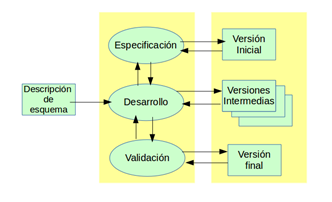
\includegraphics[width = 12 cm, height = 7 cm]{incre}
\caption{Flujo metodología incremental.}
\end{figure}

La metodología incremental, que es una pieza fundamental para enfoques ágiles, es mejor que la metodología en cascada que está más enfocada al negocio, al e-commerce y a sistemas personales. La metodología incremental refleja la manera en la que resolvemos problemas. Raramente trabajamos la solución de un problema por adelantado, pero nos movemos a través de una serie de pasos para la solución, retroalimentándonos cuando nos damos cuenta de que un error fue cometido. Desarrollar un sistema de forma incremental es barato y con un fácil manejo de cambios mientras este está siendo desarrollado.\cite{meto}\\

Cada incremento o versión del sistema incorpora una funcionalidad que necesita el cliente. Generalmente, los primeros incrementos del sistema incluyen las funcionalidades más importantes o las más urgentemente requeridas. Esto significa que el cliente puede evaluar el sistema en una etapa relativamente inicial en el desarrollo para observar si se le va a hacer entregado lo que requirió. En caso de no ser así, entonces solo el incremento tiene que cambiarse y, posiblemente se definen nuevas funcionalidades para incrementos posteriores.\\

La metodología incremental tiene tres importantes beneficios:
\begin{enumerate}
\item El costo de acomodar los cambios de requerimientos del cliente es reducido.
\item  Es más fácil obtener la retroalimentación del cliente en el desarrollo que se ha estado haciendo. Los clientes pueden comentar con base a las demostraciones del sistema y pueden ver cuanto se ha implementado. Los clientes encuentran difícil juzgar el progreso de los documentos del diseño.
\item Es posible una mayor entrega y muestra del sistema al cliente, a pesar de que no todas las funcionalidades estén incluidas.
\end{enumerate}

De alguna manera la metodología incremental es el enfoque más común para el desarrollo de aplicaciones. Este enfoque puede ser tanto dirigido por el plan como ágil o usualmente como una mezcla de enfoques. En el enfoque dirigido por el plan, los incrementos del sistema son identificados por adelantado; si un enfoque ágil es adoptado, los primeros incrementos son identificados pero el desarrollo de incrementos posteriores depende del progreso y las prioridades del cliente.\cite{meto}\\
Desde un punto de vista administrativo, la metodología incremental tiene dos problemas.

\begin{enumerate}
\item El progreso no es visible. Los administradores necesitan entregas para medir el proceso. Si el sistema es desarrollado rápidamente, no es costosamente efectivo producir documentos que reflejan cada versión del sistema.
\item La estructura del sistema se tiende a degradar cuando se agregan nuevos incrementos. A menos que el tiempo y el dinero se gaste en mejorar el sistema, cambios regulares tienden a corromper la estructura del sistema. Incorporar nuevos cambios en el software se puede convertir difícil y costoso.
\end{enumerate}

Se dividió el sistema en 3 módulos, los cuales se listan y describen a continuación.

\begin{enumerate}[{Módulo} 1.]
\item \textbf{Decodificación de DICOM.} Se decodifica  un archivo DICOM para obtener la información necesaria de la imagen.
\item \textbf{Tratamiento de imagen.} Con base a la información encontrada en el archivo DICOM se aplican diversas técnicas para detectar propiedades particulares en las tomografías. Dentro de este módulo se pueden encontrar 4 procesos principales.
\begin{enumerate}
\item Umbralización.
\item Segementación de regiones.
\item Clasificación de regiones.
\item Análisis de regiones.
\end{enumerate}
\item \textbf{Visualización.} Se presenta de manera gráfica la información contenida en un archivo de tipo DICOM permitiendo visualizar las estructuras internas del cuerpo.
\end{enumerate}

\subsection{Hardware}
Para el desarrollo del sistema se cuenta con 4 equipos de cómputo portátiles en los cuales se realizarán las implementaciones de código, pruebas y la documentación que se requiera. En la tabla 3.3 se hace una breve descripción de las características de hardware los equipos.

\begin{table}[H]
\begin{center}
\begin{tabular}{|p{30mm}|p{30mm}|p{20mm}|p{40mm}|}
\hline
 Nombre del equipo & Procesador & Memoria RAM & Sistema Operativo\\
\hline \hline 
Toshiba Satellite S40DT & AMD A8-5545 a 1.70 GHz  & 6 GB & Windows 10 Home Single Language, Elementary O.S. 0.4 Loki. 64 bits\\
\hline
Lenovo ideapad S1 5100 & Intel Core i3-3227U a 1.90 GHz & 4 GB & Windows 10 Home Single Language, Ubuntu 15.04 lts. 32 bits\\
\hline
Toshiba Satellite  & Inter Core i3-M380 a 2.53GHz  & 3 GB & Windows 8.1 pro, Ubuntu 14.04 lts. 64 bits\\
\hline
Dell Inspiron 15R & Intel Core i7 & 6 GB & Windows 10 Home Single Language de 64 bits. \\
\hline
\end{tabular}
\caption{Especificaciones de hardware}
\end{center}
\end{table}

\section{Análisis de factibilidad}
Como en todo proyecto se deben considerar ciertos factores referentes a los recursos y algunas restricciones que podrían presentarse durante el desarrollo del sistema. Se hará un estudio de factibilidad desde 3 perspectivas distintas:
\begin{itemize}
\item \textbf{Factibilidad técnica: }Se basa pincipalmente en la evaluación de los equipos tanto en software como en hardware para la realización del proyecto. Se hace también una evaluación de la infraestructura con que se cuenta para el proyecto.
\item \textbf{Factibilidad operativa: }Permite saber si es viable poner el proyecto en operación.
\item \textbf{Factibilidad económica: }Ayuda a determinar desde la perspectiva financiera si el proyecto se puede realizar, se justifican los costos y tiempos fijados con base a los beneficios que el trabajo aporta.
\end{itemize}

\subsubsection{Estudio de factibilidad operacional}
El sistema tiene una interfaz sencilla lo que permite a los usuarios tener un manejo óptimo de la herramienta para un mayor aprovechamiento de sus funciones.\\
El sistema ofrece una visualización de estructuras internas del cuerpo con gran calidad en un tiempo eficiente.\\
Se ha diseñado el sistema de manera que el usuario haga uso de este mediante una computadora portátil o de escritorio, lo cual evita el adquirir equipo de alto costo y complejidad para su manejo.\\
Con base a los usuarios potenciales de este sistema, se toma como hecho que quien haga uso de este sistema tiene conocimientos sobre las TAC, anatomía del cuerpo humano y manejo básico de computadoras.\\

\subsubsection{Estudio de factibilidad técnica}
Con base a las herramientas seleccionadas para la realización del sistema, en la tabla siguiente se listan y describen los sistemas operativos sobre los cuales se trabajará el desarrollo del sistema.
\begin{table}[H]
\begin{center}
\begin{tabular}{|p{40mm}|p{100mm}|}
\hline
Sistema & Descripción\\
\hline \hline 
Windows 8.1 Pro & Cuenta con una interfaz que permite hacer cualquier cambio sobre la PC, incluye funciones como Control de escritorio remoto, encriptado de archivos y dispositivos, Hyper-V para la creación y uso de máquinas virtuales, etc.\cite{win8}\\
\hline
Windows 10 Single Language & Sistema simple que recupera la sencillez de su interfaz, mantiene las mejores características de Windows 8 además de integrar nuevas herramientas como la visualización de multiples escritorio y la inclusión de la bash para desarrolladores.\cite{win10}\\
\hline
\end{tabular}
\caption{Sistemas operativos a utilizar.}
\end{center}
\end{table}

Tomando en cuenta los sistemas a utilizar y las herramientas se eligió utilizar el IDE Visual Studio para el desarrollo del sistema debido a la integración del framework .NET y el manejador de versiones.
\begin{table}[H]
\begin{center}
\begin{tabular}{|p{40mm}|p{100mm}|}
\hline
IDE & Descripción\\
\hline \hline 
Visual Studio & Desarrolla aplicacione para Android, iOS, Mac, Windows, la web y la nube. Escribe código con rapidez. Depurar y emitir diagnósticos fácilmente, realiza pruebas periódicas y publicar rápidamente, extender y personalizar según sus preferencias, colaboración de manera eficiente.\cite{visual}\\
\hline
\end{tabular}
\caption{IDE de desarrollo.}
\end{center}
\end{table}

Finalmente para el desarrollo de la documentación del sistema así como del manual del usuario utilizaremos Texmaker, GIMP y StarUML.
\begin{table}[H]
\begin{center}
\begin{tabular}{|p{40mm}|p{100mm}|}
\hline
 Herramienta & Descripción\\
\hline \hline 
Texmaker & Es un moderno editor de textos en Latex multiplataforma la cual conjunto una gran cantidad de funcionalidades para crear documentos en Latex en una sola aplicación.\cite{texm}\\
\hline
GIMP &  Programa de distribución libre para el retoque de fotografías, edición de la composición y creación de imágenes.\cite{gimp}\\
\hline
StarUML & Un sofisiticado modelador de software basado en las reglas de UML.\cite{star} \\
\hline
\end{tabular}
\caption{Herramientas de apoyo para documentación.}
\end{center}
\end{table}

\subsubsection{Estudio de factibilidad económica}
Para conocer el costo del sistema de deben contemplar diversos factores como el costo de los equipos para trabajar, las licencias usadas, sueldos y servicios que se requerirán durante el tiempo que se desarrolle el sistema. Es importante mencionar que 
ya se cuentas con los equipos de computo y algunas de las herramientas de software que se utilizarán, sin embargo se incluirán es este plan para hacer una estimación más cercana al precio.\\
\begin{table}[H]
\begin{center}
\begin{tabular}{|p{40mm}|p{40mm}|}
\hline
Equipo & Precio \\
\hline \hline 
Toshiba Satellite S40DT & MXN \$14,000.00\\
\hline
Lenovo ideapad S1 5100 & MXN \$8,000.00\\
\hline
Toshiba Satellite & MXN \$11,000.00 \\
\hline
Dell Inspiron 15R & MXN \$15,000.00\\
\hline \hline
Total & MXN \$48,000.00\\
\hline
\end{tabular}
\caption{Costos equipos de cómputo.}
\end{center}
\end{table}

La siguiente tabla lista los costos de los sistemas operativos que se utilizarán.

\begin{table}[H]
\begin{center}
\begin{tabular}{|p{40mm}|p{40mm}|}
\hline
Sistema operativo & Precio \\
\hline \hline 
Windows 10 Single Language & MXN \$2,499.00\\
\hline
Windows 8.1 pro & MXN \$790.00\\
\hline
Ubuntu 15.04 & Sistema de distribución libre.\cite{preubu}\\
\hline
elementary OS & Sistema de distribución libre.\cite{preele}\\
\hline \hline
Total & MXN \$8,287.00\\
\hline
\end{tabular}
\caption{Costos sistemas operativos.}
\end{center}
\end{table}

En la siguiente tabla se muestra el precio del IDE a utilizar.
\begin{table}[H]
\begin{center}
\begin{tabular}{|p{40mm}|p{40mm}|}
\hline
IDE & Precio \\
\hline \hline 
Visual Studio & Software de distribución libre en su versión Community.\cite{visual}\\
\hline \hline
Total & MXN \$0.00\\
\hline
\end{tabular}
\caption{Costos IDE.}
\end{center}
\end{table}

Se listan los precios de los softwares de apoyo junto con sus precios.

\begin{table}[H]
\begin{center}
\begin{tabular}{|p{40mm}|p{40mm}|}
\hline
Software & Precio \\
\hline \hline 
Texmaker & Software de distribución libre.\cite{texm}\\
\hline
StarUMLL & MXN Software de distribución libre.\cite{star}\\
\hline
GIMP & Sistema de distribución libre.\cite{gimp}\\
\hline \hline
Total & MXN \$0.00\\
\hline
\end{tabular}
\caption{Costos software de apoyo.}
\end{center}
\end{table}

En el desarrollo de un sistema es importante tener en cuenta los pagos de los servicios así como la renta del espacio donde se trabajará. Se hará un estimado de los gastos para un periodo de 10 meses que es el tiempo en que se tiene planeado terminar el sistema. Los costos se han obtenido con base a un promedio de los gastos de una casa con 4 habitantes.
\begin{table}[H]
\begin{center}
\begin{tabular}{|p{40mm}|p{40mm}|p{40mm}|}
\hline
Servicio/Producto & Costo mensual & Costo subtotal \\
\hline \hline 
Energía eléctrica & MXN \$350.00 & MXN \$3,500.00\\
\hline
Agua & MXN \$300.00 & MXN \$3,000.00\\
\hline
Servicio de telefonía e internet & MXN \$420.00 & MXN \$4,200.00 \\
\hline
Papelería & MXN \$150.00 & MXN \$1,500.00\\
\hline
Renta & MXN \$6,500.00 & MXN \$65,000.00 \\
\hline \hline
Total & MXN \$7720.00 & MXN \$77,200.00\\
\hline
\end{tabular}
\caption{Costos servicios.}
\end{center}
\end{table}

Ahora se muestran los gastos referentes a salarios para los desarrolladores y lider de proyecto. Con base en datos recolectados del Observatorio Laboral y la CONASAMI se establecieron los siguientes salarios para el desarrollo del proyecto.

\begin{table}[H]
\begin{center}
\begin{tabular}{|p{30mm}|p{20mm}|p{30mm}|p{30mm}|p{30mm}|}
\hline
Empleado & Numero de empleados & Salario mensual & Total de salarios Mensuales & Salarios por día \\
\hline \hline
Lider de Proyecto & 1 & MXN \$15,583.00 & MXN \$15,583.00 & MXN \$519.44\\
\hline
Programador Junior & 2 & MXN \$10,080.00 & MXN \$20,160.00 & MXN \$672.00 \\
\hline
Tester & 1 & MXN \$8,532.00 & MXN \$8,532.00 &  MXN \$284.40 \\
\hline
Limpieza & 1 & MXN \$2,000.00 & MXN \$2,000.00 & MXN \$67.00 \\
\hline \hline
Total &  &  & MXN \$46,275.00 & MXN \$1,542.84 \\
\hline
\end{tabular}
\caption{Estimación de sueldos}
\end{center}
\end{table}

Ahora para calcular el costo del proyecto en cuanto a salarios se refiere haremos un cálculo PERT.\\
El método denominado PERT ''Program Evaluation and Review Technique'' puede ser catalogado como un método cuantitativo de planificación.
El resultado final de la aplicación de este algoritmo será un cronograma para el proyecto, en el cual se podrá conocer la duración total del mismo, y la clasificación de las actividades según su criticidad. \\
Nació a finales de 1957, como resultado de un encargo de la oficina de proyectos especiales de la armada estadounidense a la división de sitemas de lockheed y a la empresa de consultoría Booz Allen \& Hamilton.\\

El PERT actúa como una herramienta para definir y coordinar lo que hay que hacer para llevar a cabo, con éxito y a tiempo, de los objetivos de un proyecto. Su campo de aplicación es tan amplio como el número de actividades susceptibles de planificación.
El PERT es un instrumento que ayuda a tomar decisiones, pero no las toma; sólo aporta información para tomarlas. Es por ello muy interesante conocer esta técnica y de ser capaz de utilizar su información, y con este fin hemos redactado este documento.\cite{pert} \\
Se consideran jornadas laborales de 8 horas, cuando se considere un tiempo de urgencia se aumentará el sueldo. Se muestra a continuación la tabla del cálculo PERT.

\begin{table}[H]
\scriptsize
\begin{center}
\begin{tabular}{|p{2.5cm}|p{1.5cm}|p{1.5cm}|p{1.5cm}|p{1.5cm}|p{1.5cm}|p{1.5cm}|}
\hline
Actividad & Marcador Actual & Marcador Anterior & Tiempo Normal & Tiempo Urgencia & Costo normal MXN & Costo urgencia MXN\\ 
\hline \hline
Desarrollo Introducción & A & & 7 & 5 &  \$10,799.88 &  \$15,428.40 \\
\hline
Desarrollo Marco Teórico & B & A & 9 & 6 &  \$13,885.56 &  \$18,514.08 \\
\hline
Diseño (Módulo decodificación imagen DICOM) & C & B & 15 & 12 &  \$23,142.60 &  \$37,028.16\\
\hline
Implementación (Módulo decodificación imagen DICOM) & D & C & 7 & 5 &  \$10,799.88 &  \$15,428.40 \\
\hline
Realizacion de pruebas (Módulo decodificación imagen DICOM) & E & C,D & 5 & 3 &  \$7,714.20 &  \$9,257.04\\ 
\hline
Diseño (Módulo tramiento de imagen) & F & E & 42 & 36 &  \$64,799.28 &  \$111,084.48\\ 
\hline
Implementación (Módulo tratamiento de imagen) & G & F & 28 & 22 &  \$43,199.52 &  \$67,884.96\\
\hline
Realizacion de pruebas (Módulo tratamiento de imagen) & H & F,G & 18 & 10 &  \$27,771.12 &  \$30,856.80\\
\hline
Diseño (Módulo visualización) & I & H & 25 & 21 &  \$38,571.00 &   \$64,799.28\\
\hline
Implementación (Módulo visualización) & J & I & 18 & 15 &  \$27,771.12 &  \$46,285.20\\
\hline
Realizacion de pruebas(Módulo visualización) & K & I,J & 13 & 8 &  \$20,056.92 &  \$24,685.44\\
\hline
\multicolumn{5}{|c|}{Costo Total} & \multicolumn{2}{|c|}{\$288,511.08}\\
\hline
\end{tabular}
\caption{Análisis PERT del sistema}
\end{center}
\end{table}

Para obtener el valor  completo del sistema se suman los costos obtenidos.
\begin{table}[H]
\begin{center}
\begin{tabular}{|p{30mm}|p{50mm}|}
\hline
Concepto & Costo\\
\hline \hline 
Hardware & MXN \$48,000.00\\
\hline
Sistemas operativos &  MXN \$8,287.00\\
\hline
Software & MXN \$0.00\\
\hline
Servicios & MXN \$77,200.00\\
\hline
Análisis PERT & MXN \$288,511.08\\
\hline \hline
Total & MXN \$421,998.08\\
\hline
\end{tabular}
\caption{Costos sistema}
\end{center}
\end{table}

Obteniendo una utilidad del 20\% se fijaría un costo de MXN \$506,397.70.


\section{Plan de manejo de riesgos}
En esta sección hablaremos sobre los riesgos y dificultades que se pueden sufrir en el desarrollo del sistema, hay que considerar cada riesgo identificado y realizar un juicio acerca de la probabilidad y gravedad de dicho riesgo y encontrar las medidas que se necesitan para poder lograr los objetivos.\\

\subsection{Identificación de riesgos}
Los riesgos identificados en la realización del sistema del trabajo terminal son:
\begin{itemize}
\item No cumplir con los objetivos principales.
\item Un integrante del equipo esté ausente por enfermedad en un momento crítico.
\item Las herramientas usadas (software) sean obsoletas.
\item Las herramientas de software no puedan trabajar en una forma íntegra.
\item Fallos en equipos de cómputo.
\item Los algoritmos no sean los adecuados conforme a lo requerido.
\item El trabajo no esté completo para la fecha de entrega.
\item No tener suficientes archivos.
\item Subestimar la complejidad del sistema.
\end{itemize}

\subsection{Análisis del riesgo}
No es posible hacer valoraciones precisas y numéricas de la probabilidad y gravedad de cada riesgo. Habrá que asignar una probabilidad del riesgo con base al criterio del equipo, a continuación se darán valores de probabilidad según la gravedad.\\\\
\begin{itemize}
\item Muy baja (menor del 10\%).
\item Baja (del 10 al 25\%).
\item Moderada (del 25 al 50\%).
\item Alta (del 50 al 75\%).
\item Muy alta (mayor del 75\%).
\end{itemize}

En la tabla 3.4 se muestra la probabilidad y el impacto que puede tener el trabajo terminal.\\

\begin{table}[H]
\begin{center}
\begin{tabular}{|p{60mm}|p{25mm}|p{25mm}|}
\hline
 Riesgo & Probabilidad & Impacto \\
\hline \hline 
No cumplir con los objetivos principales. & Muy baja. & Catastrófico.\\
\hline
Un integrante del equipo esté ausente por enfermedad en un momento crítico. & Alta. & Tolerable.\\
\hline
Las herramientas usadas (software) sean obsoletas. & Baja. & Serio.\\
\hline
Las herramientas de software nos puedan trabajar en una forma íntegra. & Moderada. & Serio.\\
\hline
Fallos en equipos de cómputo. & Alta. & Catastrófico.\\
\hline
Los algoritmos no sean los adecuados conforme a lo requerido. & Baja. & Serio. \\
\hline
El trabajo no esté completo para la fecha de entrega. & Baja. & Catastrófico.\\
\hline
No tener suficientes archivos. & Moderada. & Serio.\\
\hline
Subestimar la complejidad del sistema. & Baja. & Serio.\\
\hline
\end{tabular}
\caption{Análisis de riesgo}
\end{center}
\end{table}

\subsection{Plan de contención de riesgos}
El proceso de planeación del riesgo considera cada uno de los riesgos clave identificados y desarrolla estrategias para manejarlos. Para cada uno de los riesgos, se deberá considerar las acciones que puede tomar para minimizar la perturbación del trabajo terminal.\\

En la tabla 3.13 se muestran los riesgos y la prevención que se deben de considerar.

\begin{table}[H]
\begin{center}
\begin{tabular}{|p{70mm}|p{70mm}|}
\hline
 Riesgo & Prevención \\
\hline \hline 
No cumplir con los objetivos principales. & Tener una buena comunicación con los directores y mostrar avances del trabajo terminal continuamente.\\
\hline
Un integrante del equipo esté ausente por enfermedad en un momento crítico. & No se puede prevenir una enfermedad.\\
\hline
Las herramientas usadas (software) sean obsoletas. & Investigar si la herramienta tiene mantenimiento continuamente. \\
\hline
Las herramientas de software nos puedan trabajar en una forma íntegra. & Cuando se quiera usar una herramienta tener en cuenta si se puede integrar con las herramientas ya usadas o con herramientas que se pueden usar en el futuro.\\
\hline
Fallos en equipos de cómputo. & Tener un mantenimiento continuo de las computadoras.\\
\hline
Los algoritmos no sean los adecuados conforme a lo requerido. & Hacer una investigación a fondo de los algoritmos que se deben de usar e igual tener una variedad de algoritmos por si uno falla se tenga otros en la reserva.\\
\hline
El trabajo no esté completo para la fecha de entrega. & Cada integrante del equipo debe de hacer lo que le corresponda para poder llegar al objetivo.\\
\hline
No tener suficientes archivos. & Tener una cantidad adecuada de archivos. \\
\hline
Subestimar la complejidad del sistema. & Tener un avance continuo del proyecto y una constante revaluación del avance general del trabajo terminal.\\
\hline
\end{tabular}
\caption{Plan de contención de riesgos}
\end{center}
\end{table}


\section{Definición de requerimientos del sistema}
El objetivo principal es desarrollar una herramienta capaz de tomar un archivo DICOM almacenado en un disco donde vienen los estudios de un paciente y permita realizar un análisis y clasificación detallada de tejidos con base en los resultados obtenidos a partir del archivo DICOM.\\ 

La herramienta debe ser manipulada por el usuario (especialista) de manera muy básica, es decir, puede umbralizar, segmentar, obtener un punto creciente, clasificar (clustering) sobre un imagen DICOM.
\subsection{Requerimientos funcionales}
Los requerimientos funcionales para un sistema explican lo que el sistema debe hacer. Los requerimientos dependen del tipo de software en desarrollo, de los usuarios y del enfoque general cuando se escriben los requerimientos. Al ser los requerimientos del usuario, los requerimientos funcionales se describen por lo general de forma abstracta que entiendan los usuarios del sistema. \cite{isRF}\\ 

En la siguiente tabla 4.1 se enlistan los requerimientos funcionales del sistema.\\ 

\begin{table}[H]
\begin{center}
\begin{tabular}{|p{23mm}|p{35mm}|p{75mm}|}
\hline
 Identificador & Nombre & Descripción \\
\hline \hline 
RF1 & Seleccionar un directorio. & El usuario deberá seleccionar un directorio donde este almacenado el archivo DICOM.\\
\hline
RF2 & Visualizar imagen DICOM en 2D. & A partir del conjunto de imágenes DICOM se podrá ver la imagen sin ningún tratamiento.  \\
\hline
RF3 & Segmentar. & Para poder segmentar una parte de la imagen se hace un tratamiento adecuado para poder hacerlo.  \\
\hline
RF4 & Umbralizar. & Se umbraliza una imagen DICOM, el umbral se obtiene con base a la escala de Hounsfield para poder clasificar los tejidos.  \\
\hline
RF5 & Obtener un punto creciente. & El usuario dará una semilla (punto de origen) para buscar en su vecindad 8(celdas adyacentes a su posición), se podrá mover si hay una diferencia menor o igual a Épsilon. \\
\hline
RF6 & Clustering. & Es otra técnica para poder clasificar los diferentes tejidos que contiene la imagen DICOM. \\
\hline
RF7 & Visualizar imagen DICOM con tratamiento. & A partir de una imagen DICOM y con un tratamiento adecuado se visualizaran los tejidos.\\
\hline
\end{tabular}
\caption{Requisitos funcionales del sistema}
\end{center}
\end{table}

\subsection{Requerimientos no funcionales}
Los requerimientos no funcionales, como su nombre lo dice, son requerimientos que no se vincula directamente con las funciones específicos que el sistema proporciona. Pueden relacionarse con propiedades emergentes del sistema, como fiabilidad, tiempo de respuesta y capacidad de almacenamiento. De forma alternativa, pueden definir restricciones sobre la implementación del sistema, como las capacidades de los dispositivos I/O o las representaciones de datos
usados en las interfaces con otros sistemas. \cite{isRF} \\

En la siguiente tabla 4.2 se enlistan los requerimientos no funcionales del sistema.

\begin{table}[H]
\begin{center}
\begin{tabular}{|p{23mm}|p{35mm}|p{75mm}|}
\hline
 Identificador & Nombre & Descripción \\
\hline \hline 
RNF1 & Desarrollado en Python y C\# & Se desarrolló en estos lenguajes por dos razones la decodificación del archivo DICOM es muy sencilla en Python y por la escalabilidad que tiene C\# con otros lenguajes aunado a las herramientas de diseño proporcionadas.\\
\hline
RNF2 & Compatibilidad de lenguaje. & El compilado puede ser Python 2 o Python 3.\\
\hline
RNF3 & Intuitivo. & El sistema debe ser sencillo para el usuario que sea fácil su manejo.\\
\hline
RNF4 & Eficiente. & El tratamiento o el análisis deben ser eficiente.\\
\hline
RNF5 & Tipo de archivo. & El sistema únicamente soportara archivos DICOM.\\
\hline
RNF6 & Rapidez. & El usuario tendrá un tiempo de respuesta muy bajo cuando se le aplique una técnica a la imagen.\\
\hline
RNF7 & Actualizaciones. & El sistema debe de ser escalable para nuevas mejoras.\\
\hline
\end{tabular}
\caption{Requisitos no funcionales del sistema}
\end{center}
\end{table}

\chapter{Diseño del sistema}
\section{Arquitectura del sistema}
En esta sección describimos la entrada, núcleo y salida del sistema en un buen funcionamiento. \\
\textbf{Entrada del sistema.}\\ Para comenzar la operación del sistema se parte de una o varias imágenes DICOM con las cuales se obtiene la información necesaria para generar una visualización de un estudio tomográfico.\\
\textbf{Núcleo del sistema.}\\ Aquí se llevan a cabo todos los algoritmos sobre las regiones seleccionadas por el usuario para un mejor análisis y obtención de propiedades.\\
\textbf{Salida del sistema.}\\ Finalmente el sistema ofrece una imagen en 2D ya analizada de la región seleccionada  por el usuario, lo cual permite una mejor visualización de las estructuras.\\

\section{Casos de uso}
\subsection{Caso de uso general}

\begin{figure}[H]
\centering
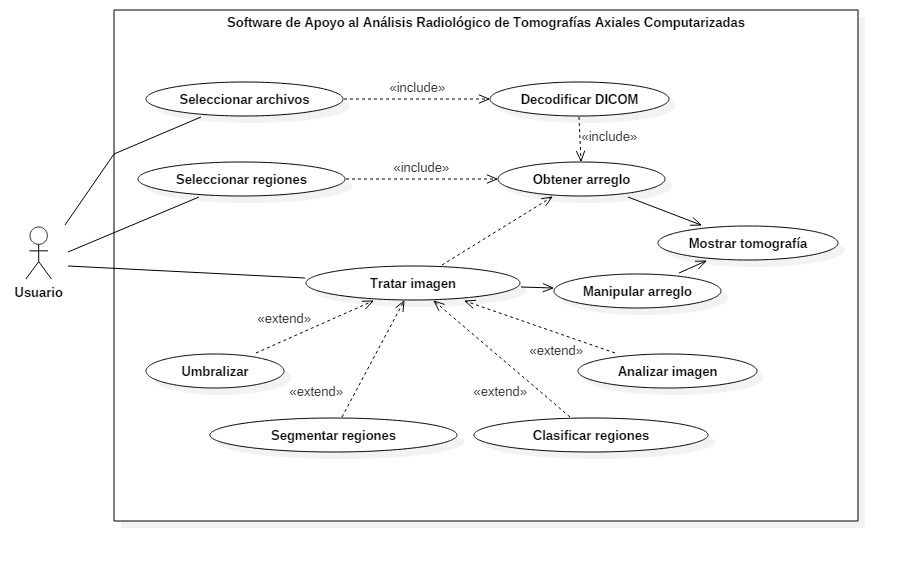
\includegraphics[width = 13 cm, height =  10 cm]{MainCasos}
\caption{Diagrama de casos de uso general.}
\end{figure}

En la figura 5.1 se observa el caso de uso general del sistema, el sistema tiene 3 interacciones principales con el usuario: selección de archivos, selección de región y tratamiento de imagen.\\ En la primera interacción el usuario a través de una interfaz selecciona uno o varios archivos en formato DICOM, una vez cargado el archivo el sistema se encargarpa de decodificar la infromación contenida para así poder generar el arreglo de valores de Hounsfield.\\ La segunda interacción principal del usuario parte de la primera, una vez que el usuario puede observar la tomografía tiene la opción de elegir una región específica, una vez acotada la región el sistema determina los valores del arreglo de Hounsfield correspondientes a la nueva región y genera una nueva matriz, posteriormente se despliega la imagen de la nueva región.\\ La tercera y útlima interacción que tiene el usuario con el sistema es el tratamiento de imágenes, para esto es necesario haber obtenido el arreglo de una región acotada, el usuario podrá realizar distintos tipos de manipulación de la imagen como umbralización, segemetación de las regiones, análisis de las regiones, incluso el análisis de la propia imagen. Una vez realizadas las operaciones necesarias el sistema se encargará de manipular el arreglo para que se puedan observar los cambios producidos sobre el estudio tomográfico.

\subsection{Caso de uso decodificación}
\begin{figure}[H]
\centering
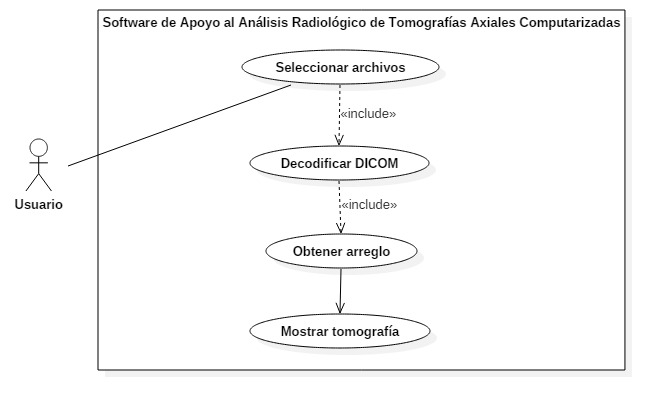
\includegraphics[width = 10 cm, height =  10 cm]{ArchivoCasos}
\caption{Diagrama caso de uso decodificación.}
\end{figure}

La figura 5.2 muestra el diagrama de caso de uso de decodificación donde el usuario elige el archivo DICOM, una vez en el sistema el archivo se decodifica y se obtiene la matriz que contiene los valores de Hounsfield y con base a esta última se muestra en 2D la tomografía.

\subsection{Caso de uso selección de región}
\begin{figure}[H]
\centering
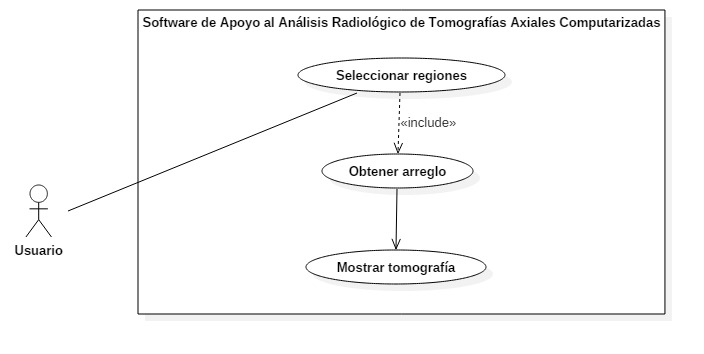
\includegraphics[width = 10 cm, height =  10 cm]{RegionCasos}
\caption{Diagrama caso de uso de selección de región.}
\end{figure}

En el caso de uso de selección de región mostrado en la figura 5.3 el usuario selecciona una región determinada para su análisis, el archivo ya se ha decodificado con aterioridad por lo que no es necesario hacerlo de nuevo, con base a la región elegida se obtiene la matriz de valores de Hounsfield correspondiente y se muestra en 2D la región seleccionada.

\subsection{Caso de uso tratamiento de imagen}
\begin{figure}[H]
\centering
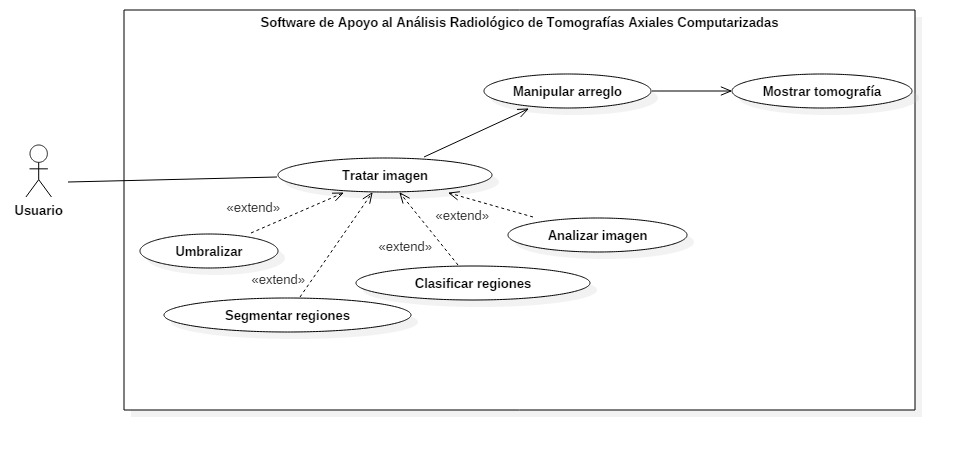
\includegraphics[width = 13 cm, height =  10 cm]{TrataCasos}
\caption{Diagrama caso de uso de tratamiento de imagen.}
\end{figure}

El caso de uso de tratamiento de imagen que se muestra en la figura 5.4 el usuario tiene la posibilidad de hacer diversas operaciones sobre la región analizada, principalmente se podrán aplicar algoritmos para umbralizar, segmentar regiones, analizar regiones y el anális de imagen, algunas operaciones que podrían entrar dentro del análisis de imagen son rotación, escalado, medición de segmentos, entre otros.

\section{Descripción de casos de uso}

\subsection{Caso de uso seleccionar archivos}
\begin{table}[H]
\begin{center}
\begin{tabular}{|p{25mm}|p{60mm}|}
\hline
Atributo & Descripción\\
\hline \hline 
Versión & 1.0\\
\hline
Actor(es) & Usuario, Sistema\\
\hline
Propósito & Dar al sistema uno o más archivos DICOM para trabajar.\\
\hline
Resumen & El usuario podra elegir uno o más archivos de tipo DICOM que se deseen estudiar.\\
\hline
Entradas & Archivos de tipo DICOM.\\
\hline
Salidas & Ruta absoluta del archivo o archivos.\\
\hline
Precondiciones & Se elige al menos un archivo de tipo DICOM.\\
\hline
Postcondiciones & Los archivos seleccionados deben ser tipo DICOM, ningún otro es válido.\\
\hline
Tipo & Primario.\\
\hline 
Módulo & 1.Módulo de decodificación de DICOM.\\
\hline
\end{tabular}
\caption{Caso de uso seleccionar archivos.}
\end{center}
\end{table}

\textbf{Flujo principal caso de uso seleccionar archivos}
\begin{enumerate}
\item El usuario elige la pestaña \textit{Archivo} y da clic en \textit{Abrir archivo}.
\item Se muestra una ventana donde el usuario puede navegar entre las carpetas y archivos existentes en el equipo.
\item El usuario selecciona el archivo o archivos DICOM.
\item El usuario da click en \textit{Aceptar}.
\item El sistema recibe la ruta del archivo de uno o varios archivos DICOM.[Alternativa A]
\item Fin del caso de uso.
\end{enumerate}

\textbf{Flujo alternativo A caso de uso seleccionar archivos. }
El usuario no selecciona ningún archivo.
\begin{enumerate}[{A}1{.}]
\item No se recibe ninguna ruta.
\item Se manda un mensaje de error.
\item Se despliega la ventana con las carpetas y archivos del equipo.
\item El usuario selecciona el archivo o archivos DICOM.
\item El usuario da click en \textit{Aceptar}.
\item El sistema recibe la ruta del archivo de uno o varios archivo DICOM.
\item Fin del caso de uso.
\end{enumerate}

\subsection{Caso de uso decodificar DICOM}
\begin{table}[H]
\begin{center}
\begin{tabular}{|p{25mm}|p{60mm}|}
\hline
Atributo & Descripción\\
\hline \hline 
Versión & 1.0\\
\hline
Actor(es) & Sistema\\
\hline
Propósito & Decodificar un archivo de tipo DICOM para obtener los valores de Hounsfield.\\
\hline
Resumen & El sistema decodifica el archivo o archivos DICOM seleccionados por el usuario anteriormente.\\
\hline
Entradas & Archivos DICOM.\\
\hline
Salidas & Valores de Hounsfield.\\
\hline
Precondiciones & El archivo cargado es tipo DICOM.\\
\hline
Postcondiciones & Los valores obtenidos están dentro de los rangos de la escala de Hounsfield.\\
\hline
Tipo & Primario.\\
\hline 
Módulo & 1.Módulo de decodificación de DICOM.\\
\hline
\end{tabular}
\caption{Caso de uso decodificar DICOM.}
\end{center}
\end{table}

\textbf{Flujo principal caso de uso decodificar DICOM}
\begin{enumerate}
\item El sistema accede a la ruta absoluta del archivo.
\item El sistema valida que el archivo sea tipo DICOM.[Ruta alternatvia A]
\item Se crea un objeto DICOM.
\item Se almacena la información contenida en el archivo DICOM.
\item Fin del caso de uso.
\end{enumerate}

\textbf{Flujo alternativo A caso de uso decodificar DICOM. }
El usuario no selecciona ningún archivo.
\begin{enumerate}[{A}1{.}]
\item El archivo no es de tipo DICOM.
\item Se manda un mensaje de error.
\item Se despliega la ventana con las carpetas y archivos del equipo.
\item El usuario selecciona el archivo o archivos DICOM.
\item Se lee y verifica que el archivo sea tipo DICOM.[Ruta alternatvia A]
\item Se crea un objeto DICOM.
\item Se almacena la información contenida en el archivo DICOM.
\item Fin del caso de uso.
\end{enumerate}

\subsection{Caso de uso obtener arreglo}
\begin{table}[H]
\begin{center}
\begin{tabular}{|p{25mm}|p{60mm}|}
\hline
Atributo & Descripción\\
\hline \hline 
Versión & 1.0\\
\hline
Actor(es) & Sistema\\
\hline
Propósito & Ordenar los valores de Hounsfield.\\
\hline
Resumen & El sistema almacena en un arreglo los valores de Hounsfield obtenidos de la imagen.\\
\hline
Entradas & Conjunto de valores decodificados.\\
\hline
Salidas & Arreglo con los valores de Hounsfield.\\
\hline
Precondiciones & El archivo DICOM fue decodificado.\\
\hline
Postcondiciones & El arreglo contiene unicamente valores dentro de los rangos de la escala de Hounsfield.\\
\hline
Tipo & Primario.\\
\hline 
Módulo & 1.Módulo de decodificación de DICOM.\\
\hline
\end{tabular}
\caption{Caso de uso obtener arreglo.}
\end{center}
\end{table}

\textbf{Flujo principal caso obtener arreglo. }
\begin{enumerate}
\item El sistema lee los valores obtenidos en la decodificación.
\item Se obtienen los valores correspondientes a cada segmento de la tomografía.
\item Se organizan los valores en una matriz.
\item Fin del caso de uso.
\end{enumerate}

\subsection{Caso de uso seleccionar región}
\begin{table}[H]
\begin{center}
\begin{tabular}{|p{25mm}|p{60mm}|}
\hline
Atributo & Descripción\\
\hline \hline 
Versión & 1.0\\
\hline
Actor(es) & Usuario, Sistema\\
\hline
Propósito & Acotar una región para su tratamiento.\\
\hline
Resumen & El usuario elige acotar una región y mediante una herramienta proporcionada por el sistema se selecciona lo que se desea analizar.\\
\hline
Entradas & Conjunto de cordenadas que comprenden la región.\\
\hline
Salidas & Conjunto de valores de Hounsfield correspondientes a la región.\\
\hline
Precondiciones & La imagen ya fue decodificada y el arreglo obtenido.\\
\hline
Postcondiciones & El arreglo contiene unicamente valores dentro de los rangos de la escala de Hounsfield.\\
\hline
Tipo & Primario.\\
\hline 
Módulo &  1.Módulo de decodificación de DICOM.\\
\hline
\end{tabular}
\caption{Caso de uso seleccionar región.}
\end{center}
\end{table}

\textbf{Flujo principal caso seleccionar región. }
\begin{enumerate}
\item El usuario activa la opción \textit{Acotar región}.
\item El sistema proporciona al usuario una herramienta para la delimitación de un área.
\item El usuario delimita la región que desea analizar.
\item El sistema valida que la región esté dentro de los límites de la tomografía.[Flujo alternativo A.]
\item Se dan los valores correspondientes al área acotada.
\item Fin del caso de uso.
\end{enumerate}

\textbf{Flujo alternativo A caso de uso seleccionar región. }
El usuario no selecciona ningún archivo.
\begin{enumerate}[{A}1{.}]
\item Uno de los límites de la región sale de al área válida.
\item Se manda un mensaje de error.
\item Se reposiciona la herramienta de acotación.
\item El usuario delimita la región que desea analizar.
\item El sistema valida que la región esté dentro de los límites de la tomografía.
\item Se dan los valores correspondientes al área acotada.
\item Fin del caso de uso.
\end{enumerate}

\subsection{Caso de uso tratar imagen}
\begin{table}[H]
\begin{center}
\begin{tabular}{|p{25mm}|p{60mm}|}
\hline
Atributo & Descripción\\
\hline \hline 
Versión & 1.0\\
\hline
Actor(es) & Usuario, Sistema\\
\hline
Propósito & Permitir al usuario realizar un conjunto de operaciones sobre la imagen.\\
\hline
Resumen & El usuario elige la operación que se hará sobre la imagen.\\
\hline
Entradas & Operación a realizar.\\
\hline
Salidas & Valores tratados.\\
\hline
Precondiciones & La imagen ya fue decodificada y el arreglo obtenido.\\
\hline
Postcondiciones & Los valores tratados respetan la escala de Hounsfield.\\
\hline
Tipo & Secundario.\\
\hline 
Módulo & 2.Tratamiento de imagen.\\
\hline
\end{tabular}
\caption{Caso de uso tratar imagen.}
\end{center}
\end{table}

\textbf{Flujo principal caso tratar imagen. }
\begin{enumerate}
\item El usuario elije el tratamiento que desea aplicar.
\item El sistema aplica los algoritmos requeridos a cada proceso.
\item Se generan los valores correspondientes obteniendo nuevos datos.
\item Fin del caso de uso.
\end{enumerate}

\subsection{Caso de uso umbralizar}
\begin{table}[H]
\begin{center}
\begin{tabular}{|p{25mm}|p{60mm}|}
\hline
Atributo & Descripción\\
\hline \hline 
Versión & 1.0\\
\hline
Actor(es) & Usuario, Sistema\\
\hline
Propósito & Umbralizar la imagen para obtener propiedades no visibles.\\
\hline
Resumen & El sistema aplica algoritmos de umbralización con base a las propiedades de la imagen.\\
\hline
Entradas & Arreglo a umbralizar.\\
\hline
Salidas & Imagen umbralizada.\\
\hline
Precondiciones & La imagen ya fue decodificada y el arreglo obtenido.\\
\hline
Postcondiciones & Los valores están dentro de la escala de Hounsfield.\\
\hline
Tipo & Primario.\\
\hline 
Módulo & 2.Tratamiento de imagen.\\
\hline
\end{tabular}
\caption{Caso de uso umbralizar.}
\end{center}
\end{table}

\textbf{Flujo principal caso umbralizar. }
\begin{enumerate}
\item El usuario selecciona la opción \textit{Umbralizar}.
\item El sistema lee la matriz de la región a umbralizar.
\item Se aplica una serie de algoritmos.
\item Se obtienen los valores umbralizados.
\item Fin del caso de uso.
\end{enumerate}

\subsection{Caso de uso segementar regiones}
\begin{table}[H]
\begin{center}
\begin{tabular}{|p{25mm}|p{60mm}|}
\hline
Atributo & Descripción\\
\hline \hline 
Versión & 1.0\\
\hline
Actor(es) & Usuario, Sistema\\
\hline
Propósito & Segmentar una o varias regiones.\\
\hline
Resumen & Se aplican los algoritmos requeridos para una segmentación.\\
\hline
Entradas & Arreglo de valores de Hounsfield.\\
\hline
Salidas & Valores segementados.\\
\hline
Precondiciones & La imagen ya fue decodificada y el arreglo obtenido.\\
\hline
Postcondiciones & Valores tratados respetan la escala de Hounsfield.\\
\hline
Tipo & Primario.\\
\hline 
Módulo & 2.Tratamiento de imagen.\\
\hline
\end{tabular}
\caption{Caso de uso segmentar regiones.}
\end{center}
\end{table}

\textbf{Flujo principal caso segmentar regiones. }
\begin{enumerate}
\item El usuario selecciona la opción \textit{Segmentar}.
\item El sistema aplica los algoritmos requeridos.
\item Se obtienen los valores de la segmentación.
\item Fin del caso de uso.
\end{enumerate}

\subsection{Caso de uso clasificar regiones}
\begin{table}[H]
\begin{center}
\begin{tabular}{|p{25mm}|p{60mm}|}
\hline
Atributo & Descripción\\
\hline \hline 
Versión & 1.0\\
\hline
Actor(es) & Usuario, Sistema\\
\hline
Propósito & Clasificar las regiones con base a distintos criterios.\\
\hline
Resumen & Se aplican los algoritmos requeridos para una clasificación dependiendo el criterio.\\
\hline
Entradas & Arreglo de valores de Hounsfield.\\
\hline
Salidas & Valores clasificados.\\
\hline
Precondiciones & La imagen ya fue decodificada y el arreglo obtenido.\\
\hline
Postcondiciones & Valores tratados respetan la escala de Hounsfield.\\
\hline
Tipo & Primario.\\
\hline 
Módulo & 2.Tratamiento de imagen.\\
\hline
\end{tabular}
\caption{Caso de uso clasificar regiones.}
\end{center}
\end{table}

\textbf{Flujo principal caso clasificar regiones. }
\begin{enumerate}
\item El usuario selecciona la opción \textit{Clasificar}.
\item El sistema aplica los algoritmos dependiendo el criterio de clsaificación.
\item Se clasifican los distintos valores.
\item Fin del caso de uso.
\end{enumerate}

\subsection{Caso de uso analizar regiones}
\begin{table}[H]
\begin{center}
\begin{tabular}{|p{25mm}|p{60mm}|}
\hline
Atributo & Descripción\\
\hline \hline 
Versión & 1.0\\
\hline
Actor(es) & Usuario, Sistema\\
\hline
Propósito & Aplicar operaciones especificas sobre la imagen.\\
\hline
Resumen & Se aplican operaciones de menor complejidad.\\
\hline
Entradas & Arreglo de valores de Hounsfield y dependiendo la operación los parámtros necesarios.\\
\hline
Salidas & Valores manipulados.\\
\hline
Precondiciones & La imagen ya fue decodificada y el arreglo obtenido.\\
\hline
Postcondiciones & La imagen mantiene su integridad.\\
\hline
Tipo & Secundario.\\
\hline 
Módulo & 2.Tratamiento de imagen.\\
\hline
\end{tabular}
\caption{Caso de uso analizar regiones.}
\end{center}
\end{table}

\textbf{Flujo principal caso analizar regiones. }
\begin{enumerate}
\item El usuario selecciona la operación deseada, como pueden ser \textit{Rotar}, \textit{Escalar}, \textit{Medir}, entre otras.
\item El usuario proporciona los parámetros necesarios.
\item Se aplica la operación.
\item Se devuelve el resultado de aplicar la operación.
\item Fin del caso de uso.
\end{enumerate}


\subsection{Caso de uso manipular arreglo}
\begin{table}[H]
\begin{center}
\begin{tabular}{|p{25mm}|p{60mm}|}
\hline
Atributo & Descripción\\
\hline \hline 
Versión & 1.0\\
\hline
Actor(es) & Sistema\\
\hline
Propósito & Asignar los nuevos valores a la matriz sin perder la información.\\
\hline
Resumen & Se asignan los valores nuevos a las matrices cuidando la integridad de las demás.\\
\hline
Entradas & Valores de Hounsfield.\\
\hline
Salidas & Arreglo manipulado.\\
\hline
Precondiciones & La imagen ya fue decodificada y el arreglo obtenido.\\
\hline
Postcondiciones & La imagen mantiene su integridad.\\
\hline
Tipo & Primario.\\
\hline 
Módulo & 2.Tratamiento de imagen.\\
\hline
\end{tabular}
\caption{Caso de uso manipular arreglo.}
\end{center}
\end{table}

\textbf{Flujo principal caso manipular arreglo. }
\begin{enumerate}
\item Se trata la imagen.
\item Se envía el conjunto de valores ya tratados.
\item Se guardan en la nueva matriz.
\item Fin del caso de uso.
\end{enumerate}

\subsection{Caso de uso mostrar tomgrafía}
\begin{table}[H]
\begin{center}
\begin{tabular}{|p{25mm}|p{60mm}|}
\hline
Atributo & Descripción\\
\hline \hline 
Versión & 1.0\\
\hline
Actor(es) & Sistema\\
\hline
Propósito & Mostrar la tomografía al usuario.\\
\hline
Resumen & Con base a los valores de Hounsfield se genera la visualización de la tomografía en 2D.\\
\hline
Entradas & Arreglo con valores de Hounsfield.\\
\hline
Salidas & Imagen en 2D de la tomografía.\\
\hline
Precondiciones & La imagen ya fue decodificada y el arreglo obtenido.\\
\hline
Postcondiciones & La matriz de Hounsfield no se desecha, se guarda para usos posteriores.\\
\hline
Tipo & Primario.\\
\hline 
Módulo & 3.Visualización.\\
\hline
\end{tabular}
\caption{Caso de uso mostrar tomografía.}
\end{center}
\end{table}

\textbf{Flujo principal caso mostrar tomografía. }
\begin{enumerate}
\item Se recibe el arreglo de valores de Hounsfield.
\item Se genera la visualización de la tomografía en 2D.
\item Fin del caso de uso.
\end{enumerate}

\section{Diagramas de secuencia}
\subsection{Secuencia: Decodificar DICOM}
\begin{figure}[H]
\centering
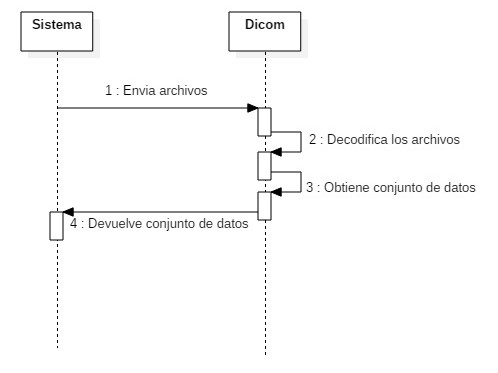
\includegraphics[width = 12 cm, height = 7 cm]{Decodificar}
\caption{Secuencia:Decodificar DICOM.}
\end{figure}

\subsection{Secuencia: Seleccionar archivos}
\begin{figure}[H]
\centering
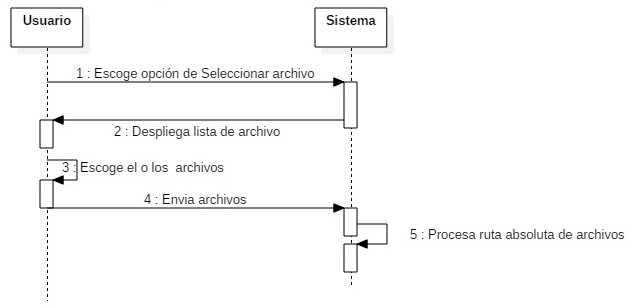
\includegraphics[width = 12 cm, height = 7 cm]{seleccionar_archivo}
\caption{Secuencia:Seleccionar archivos.}
\end{figure}

\subsection{Secuencia: Obtener arreglo}
\begin{figure}[H]
\centering
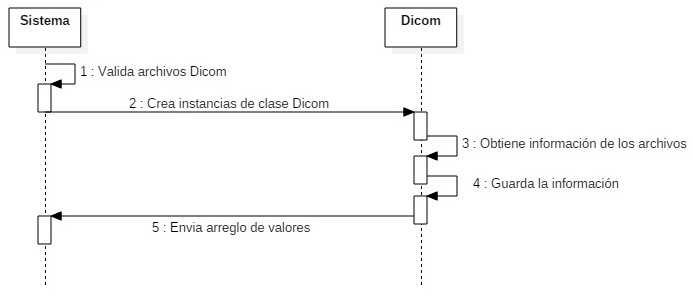
\includegraphics[width = 12 cm, height = 7 cm]{obtener_arreglo}
\caption{Secuencia:Obtener arreglo.}
\end{figure}

\subsection{Secuencia: Seleccionar regiones}
\begin{figure}[H]
\centering
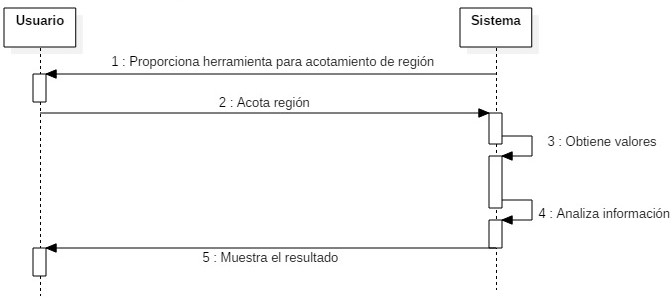
\includegraphics[width = 12 cm, height = 7 cm]{region}
\caption{Secuencia:Seleccionar regiones.}
\end{figure}

\subsection{Secuencia: Analizar imagen}
\begin{figure}[H]
\centering
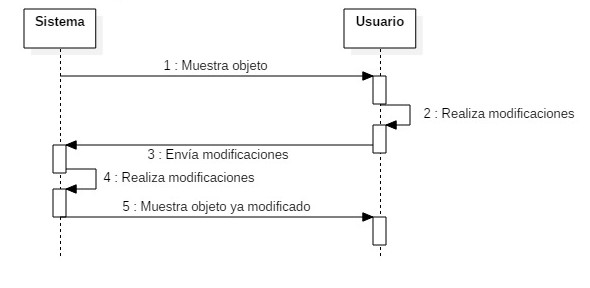
\includegraphics[width = 12 cm, height = 7 cm]{analisis}
\caption{Secuencia:Analizar imagen.}
\end{figure}

\subsection{Secuencia: Clasificar regiones}
\begin{figure}[H]
\centering
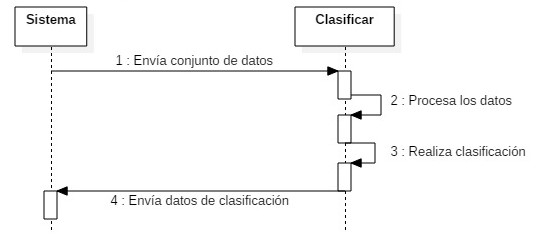
\includegraphics[width = 12 cm, height = 7 cm]{clasificacion}
\caption{Secuencia:Clasificar regiones.}
\end{figure}

\subsection{Secuencia: Manipular arreglo}
\begin{figure}[H]
\centering
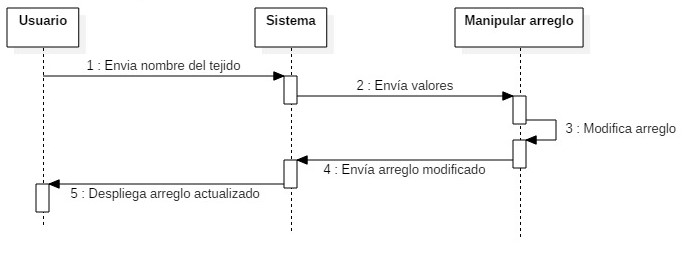
\includegraphics[width = 12 cm, height = 7 cm]{modificar_arreglo}
\caption{Secuencia:Manipular arreglo.}
\end{figure}

\subsection{Secuencia: Segmentar regiones}
\begin{figure}[H]
\centering
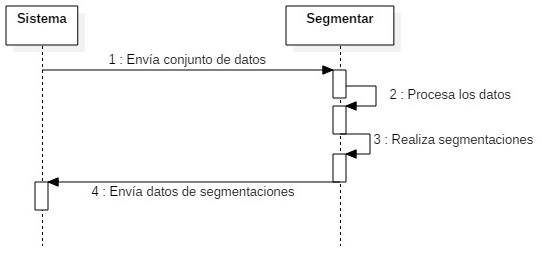
\includegraphics[width = 12 cm, height = 7 cm]{segmentacion}
\caption{Secuencia:Segmentar regiones.}
\end{figure}

\subsection{Secuencia: Tratar imagen}
\begin{figure}[H]
\centering
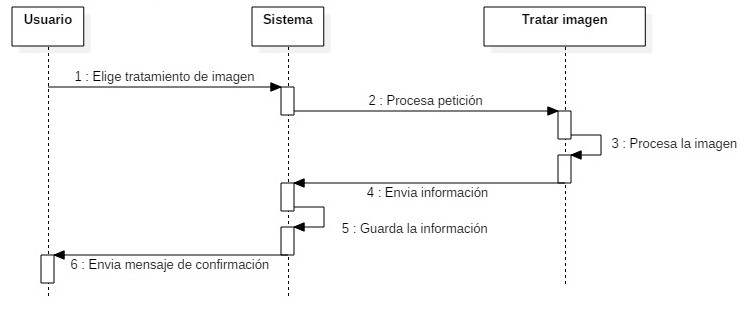
\includegraphics[width = 12 cm, height = 7 cm]{tratamiento}
\caption{Secuencia:Tratar imagen.}
\end{figure}

\subsection{Secuencia: Umbralizar}
\begin{figure}[H]
\centering
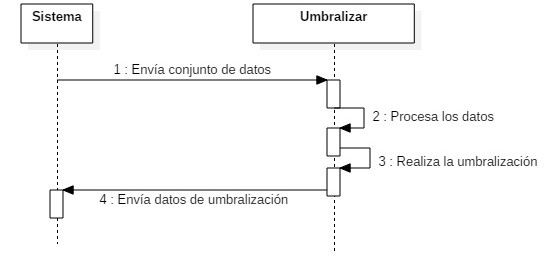
\includegraphics[width = 12 cm, height = 7 cm]{umbralizacion}
\caption{Secuencia:Umbralizar.}
\end{figure}

\subsection{Secuencia: Mostrar tomografía}
\begin{figure}[H]
\centering
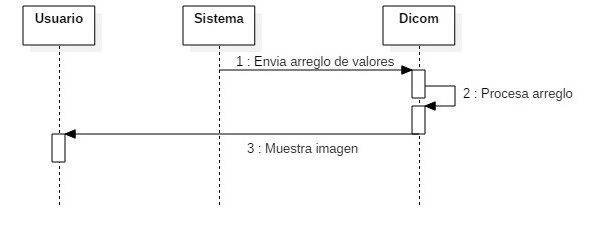
\includegraphics[width = 12 cm, height = 7 cm]{mostrar_tomografia}
\caption{Secuencia:Mostrar tomografía.}
\end{figure}


\chapter{Desarrollo}
En este capítulo se explican cuales fueron los algoritmos elegidos para el sistema, donde se utilizan, se explica como fue su implementación y cómo se modifican los parámetros en cada uno para obtener diferentes resultados.

\section{Decodificación de DICOM}
Para la decodificación de los archivos DICOM se hace uso de la función \textit{dicom.read\_file} encontrada en la librería \textit{PYDICOM} del lenguaje Python, la cual al enviarle la ruta de la carpeta donde se encuentran los archivos DICOM nos permite obtener toda la información de cada uno. Una de las etiquetas propias de la librería es  el atributo \textit{pixel\_array}, el cual nos devuelve la matriz de densidades. Utilizando las etiquetas estandarizadas en DICOM podemos obtener los datos que deseemos. Algunos ejemplos de las etiquetas utilizadas son:

\begin{table}[H]
\begin{center}
\begin{tabular}{|p{30mm}|p{40mm}|}
\hline
Etiqueta & Parámetro obtenido\\
\hline \hline 
0X28, 0X30 & Distancia entre centros de pixeles\\
\hline
0X10, 0X10 & Nombre del paciente\\
\hline
0X10, 0X1010 & Edad del paciente\\
\hline
0X10, 0X40 & Sexo del paciente\\
\hline
0X8, 0X20 & Fecha de toma del estudio\\
\hline
0X18, 0X50 & Espesor de tomografía\\
\hline
0X08, 0X08 & Hospital o clínica donde fue tomado el estudio\\
\hline
\end{tabular}
\caption{Etiquetas DICOM usadas en el sistema.}
\end{center}
\end{table}

\section{Comunicación entre lenguajes}
Para una mejor implementación del sistema se usan 2 lenguajes, lo cual nos lleva a la tarea de enviar información entre ellos. El framework .NET nos facilita esta tarea mediante el uso de procesos, con funciones basadas en arquitectura tipo \textit{pipelines}, esta arquitectura permite que los procesos creados accedan a otro programa y el flujo de datos generado en ese programa se conserve en el proceso padre.\\

La arquitectura se pudo implementar gracias a la librería \textit{System.Diagnostics} que nos da acceso a objetos de tipo \textit{ProcessStartInfo} dentro del framework .NET, se hace uso de funciones como \textit{UseShellExecute} para iniciar la ejecución de un programa desde los procesos creados y \textit{RedirectStandardOutput} para leer el flujo de datos.

\section{Umbralización}
La naturaleza de la TAC nos permite obtener una matriz de densidades. Gracias a la clasificación propuesta por Hounsfield se parametrizan los órganos y tejidos teniendo un valor y una ventana de tolerancia en cada uno. Tomando los valores de la escala de Hounsfield se procedió a implementar una umbalización por definición. Una vez que se ha elegido el tejido que se desea visualizar se recorre toda la matriz de densidades y se hace un mapeo con un color distinto cuando el valor de pixel se encuentra dentro  del rango definido por la escala.\\
Los tejidos que es posible visualizar en el sistema son \textit{agua, aire, fluido cerebroespinal, sustancia cerebral blanca, sustancia cerebral gris, grasa, hueso compacto, hueso esponjoso, hígado, páncreas, pulmón, riñón, sangre y sangre coagulada}.

\section{Segmentación}
La segementación en este sistema tiene como intención el poder aislar los tejidos entre si. Para estos procedimientos se recurrió  a dos técnicas de segmentación distintas, la primera de ellas es la técnica \textit{Región creciente}, la cual requiere de una interación con el usuario; la otra ténica utilizada es \textit{Split and merge} la cual no requiere de ninguna interacción para su funcionamiento.

\subsection{Región creciente}
El algoritmo \textit{Región creciente} nos permite encontrar la continuidad de un tejido seleccionado por el usuario. Una vez que el usuario selecciona el punto, se inicia una busqueda de amplitud con parámetros de similitud basados en distancia Euclidiana y proximidad al punto de origen, encontrando así pixeles con características similares entre si con el fin de formar un objeto.

\subsection{Split and merge}
\textit{Split and merge} nos permite agrupar objetos(tejidos) con características de similitud basadas en su UH y la proximidad entre los pixeles. Una de la ventajas de utilizar este método a diferencia del algoritmo de \textit{Región creciente} es que aquí no se tiene un punto de partida sobre el cual hacer la busqueda por lo que tenemos una mayor área para encontrar objetos sin embargo esto puede significar un problema para la delimitación de diferentes objetos debido a la abundante cantidad de datos presente.


\section{Clasificación}
Los clasificadores nos permiten agrupar pixeles con características similares, se hicieron 2 implementaciones para cada uno de los algoritmos elegidos, una  supervisada y una no supervisada, en ambas implementaciones el usuario tiene la opción de definir el número de grupos que desea encontrar en la TAC. En la implementación supervisada el usuario define los centros de cada grupo.

\subsection{K-means}
Se implementó el algoritmo \textit{K-means}para la creación de grupos dentro de la TAC, se usa la distancia Euclidiana entre pixeles como parámetro de similitud. La distancia Euclidiana es calculada con base a las densidades de los tejidos. Este algoritmo es muy útil cuando se buscan grupos cuya deifnición no se encuentra dentro del conjunto de información.

\subsection{Fuzzy C-Means}
El algoritmo \textit{Fuzzy C-Means} trabaja de manera similar al algoritmo anteriorpero en este la diferencia entre pixeles es menos tolerable dando así un valor más definido de similitud. Además se cuenta con una matriz de pertenencia la cual nos ayuda a identificar el cluster al que pertenece el pixel analizado. La matriz da un valor a cada cluster para cada pixel y se elige el que mayor pertenencia tiene.

\chapter{Pruebas}
En este capítulo se muestran los diferentes resultados obtenidos durante el funcionamiento del sistema. Para poder llevar acabo estas pruebas de funcionamiento se utilizaron TAC proporcionadas por uno de nuestros directores. En los estudios podemos observar desde el cerebro hasta los pies de diversos pacientes lo cual enriquece estas pruebas y nos permite tener una mayor perspectiva al momento de hacer una autoevaluación del sistema.

\section{Umbralización}
Las imágenes mostradas a continuación corresponden a diferentes umbralizaciones realizadas con el sistema.

\newpage
\vspace*{3cm}
En la umbralización de fluido cerebro espinal se utilizó un TAC obtenida de la zona de la cabeza de un paciente. Teniendo del lado derecho la tomografía sin ningún tratamiento y del lado izquierdo la imagen tratada el fluido puede observarse con un tono verde.  
\begin{figure}[H]
\centering
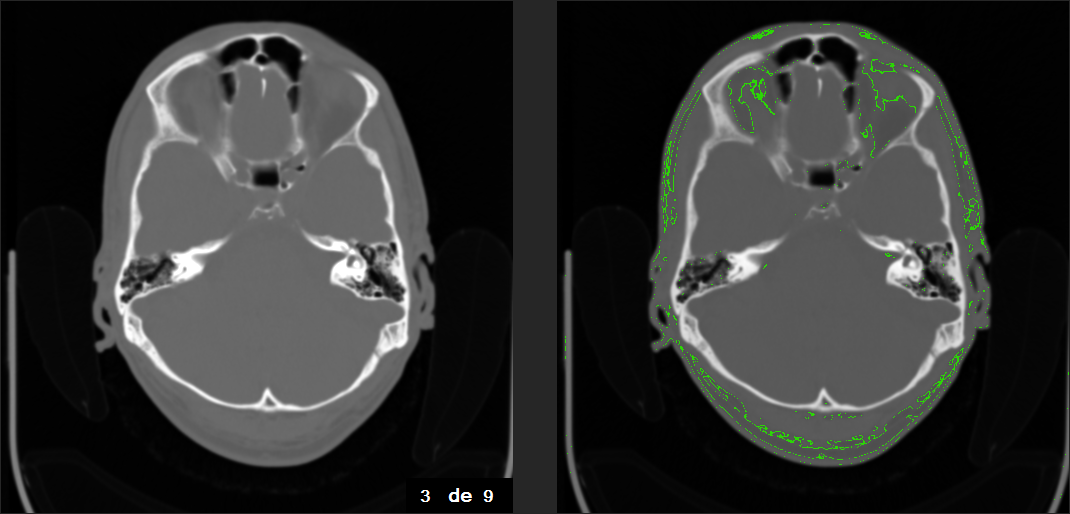
\includegraphics[width = 15 cm, height = 8 cm]{umbralFluidoCerebralEspinal}
\caption{Umbralización de fluido cerebro espinal.}
Captura de pantalla del sistema en funcionamiento.
\end{figure}

\newpage
\vspace*{3cm}
Para la umbralización del tejido graso se utilizó una tomografía de la zona abdominal, en esta zona es donde mayor acumulación de grasa hay regularmente, en otras zonas del cuerpo podemos observar este tejido en la piel.
\begin{figure}[H]
\centering
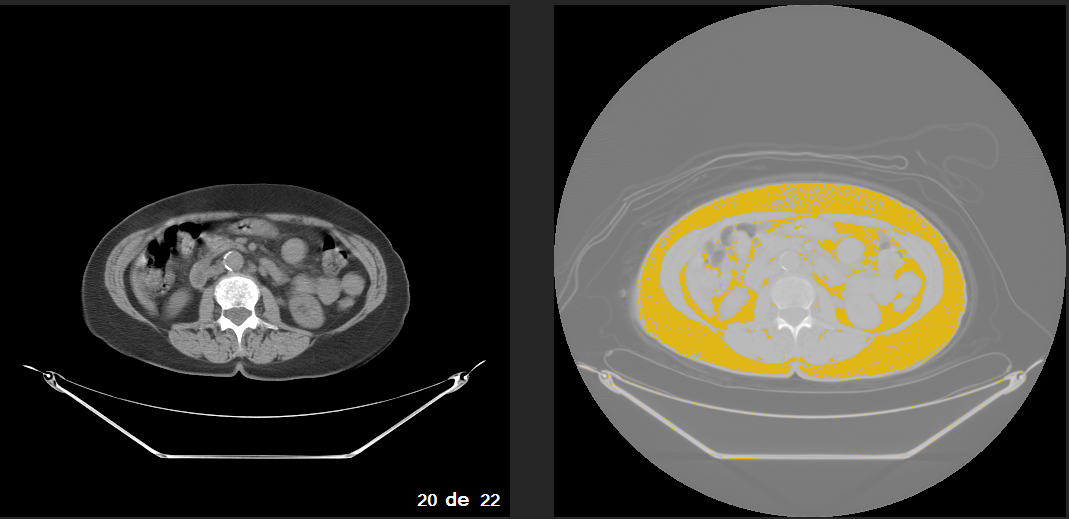
\includegraphics[width = 15 cm, height = 8 cm]{umbralGrasa}
\caption{Umbralización de grasa.}
Captura de pantalla del sistema en funcionamiento.
\end{figure}

\newpage
\vspace*{3cm}
En la umbralización de los pulmones podemos observar que no es una figura muy solida y el tejido es muy similar al aire debido al contenido de estos órganos.
\begin{figure}[H]
\centering
\includegraphics[width = 15 cm, height = 8 cm]{umbralPulmon}
\caption{Umbralización de pulmón.}
Captura de pantalla del sistema en funcionamiento.
\end{figure}

\newpage
\vspace*{3cm}
Continuando con la tomografría de zona abdominal se realizó una umbralización para hueso compacto, donde únicamente podemos ver lo correspondiente a la columna vertebral con un tono rosaceo del lado izquierdo.
\begin{figure}[H]
\centering
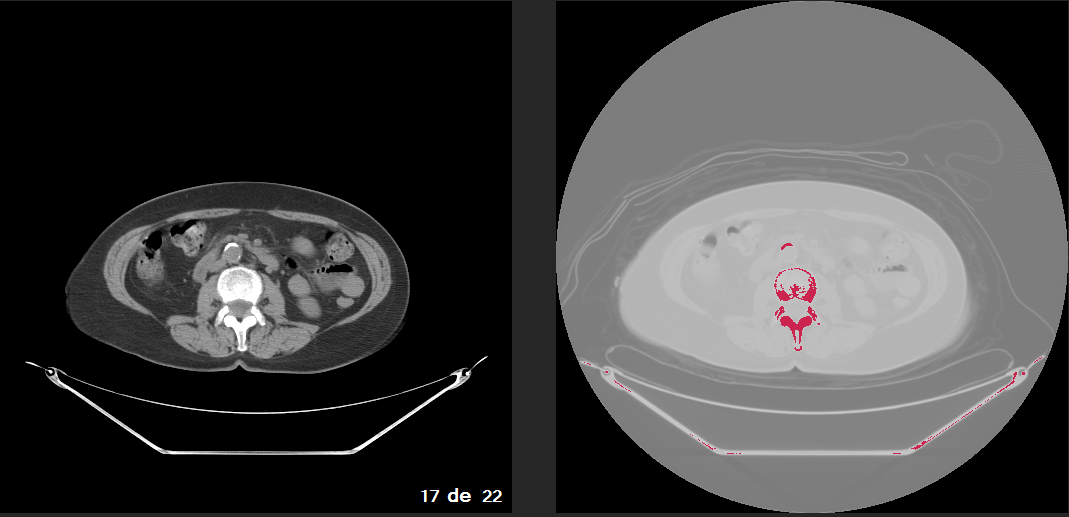
\includegraphics[width = 15 cm, height = 8 cm]{umbralHuesoCompacto}
\caption{Umbralización de hueso compacto.}
Captura de pantalla del sistema en funcionamiento.
\end{figure}

\newpage
\vspace*{3cm}
A diferencia del estudio utilizado para el hueso compacto en el hueso esponjoso se utlizó un estudio cerebral donde podemos ver la protección que el craneo da al cerebro, el hueso esponjoso regularmente se combina con hueso compacto.
\begin{figure}[H]
\centering
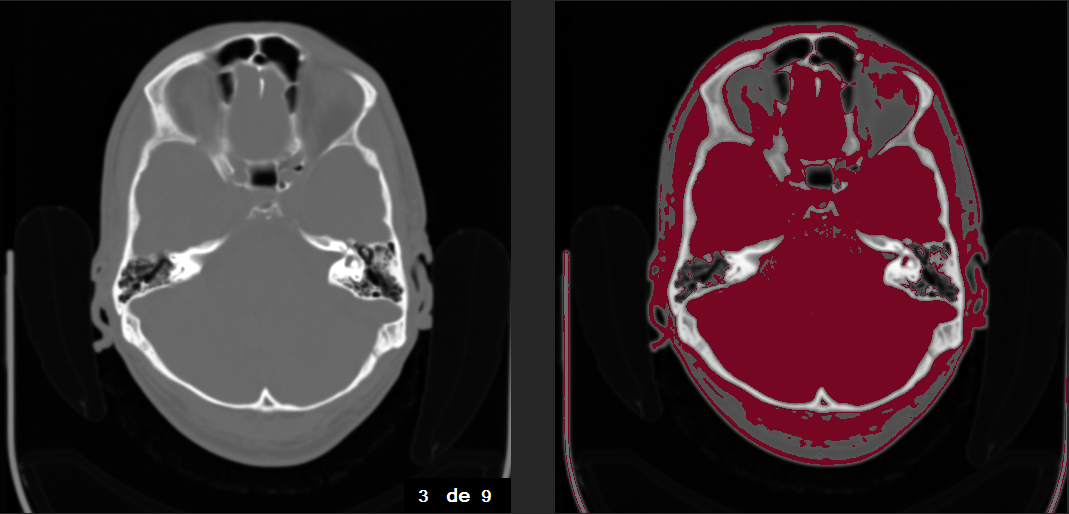
\includegraphics[width = 15 cm, height = 8 cm]{umbralHuesoEsponjoso}
\caption{Umbralización de hueso esponjoso.}
Captura de pantalla del sistema en funcionamiento.
\end{figure}

\newpage
\vspace*{3cm}
La umbralización de sangre se realizó sobre una tomografía de cerebro, el cerebro está inundado de diferentes fluidos por lo cual no observaremos una gran continuidad como se puede ver en el hueso esponjoso.
\begin{figure}[H]
\centering
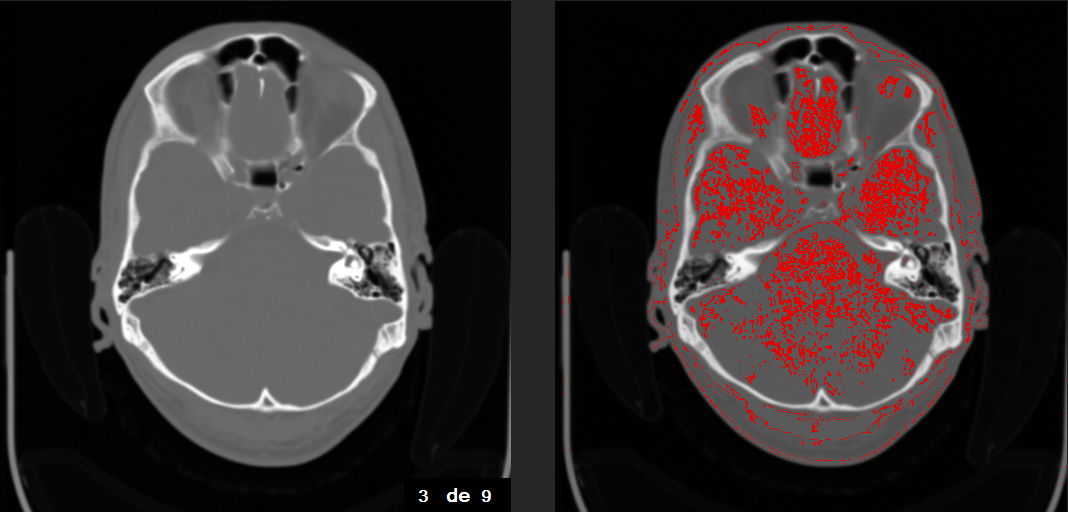
\includegraphics[width = 15 cm, height = 8 cm]{umbralSangre}
\caption{Umbralización de sangre.}
Captura de pantalla del sistema en funcionamiento.
\end{figure}

\newpage
\vspace*{3cm}
Otro fluido importante que encontramos en el cerebro es la sustancia cerebral gris, esta se encuentra en una menor proporción que la sangre.
\begin{figure}[H]
\centering
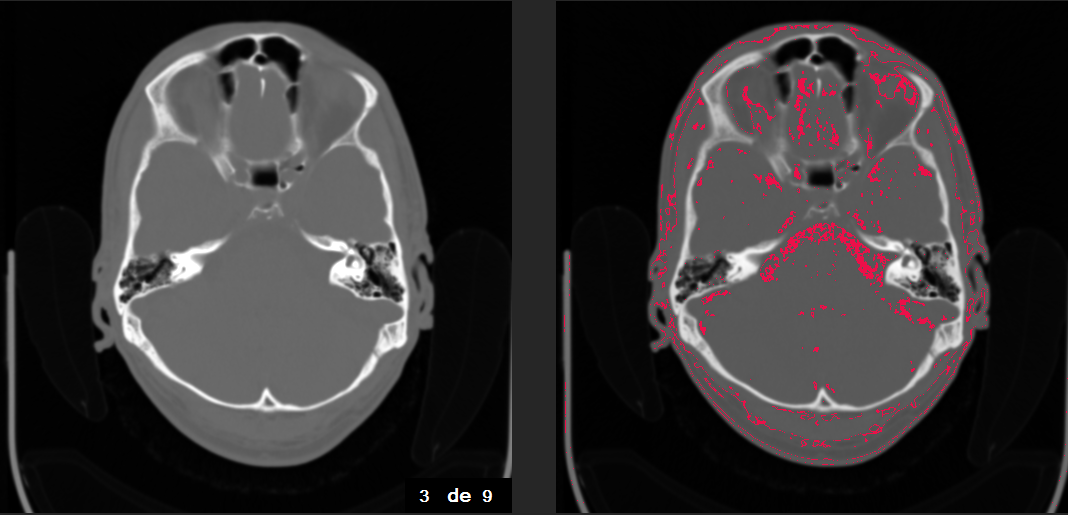
\includegraphics[width = 15 cm, height = 8 cm]{umbralSustanciaCerebralGris}
\caption{Umbralización de sustancia cerebral gris.}
Captura de pantalla del sistema en funcionamiento.
\end{figure}

\newpage
\section{Contraste}
Las herramientas de contraste en los visores DICOM son muy importantes pues permiten obtener un mayor detalle de las estructuras internas del cuerpo sin hacer un tratamiento sobre la TAC, en este caso se hace un mapeo con la escala de gris para dar más o menos valores a cada tejido.
\vspace{2cm}
\begin{figure}[H]
\centering
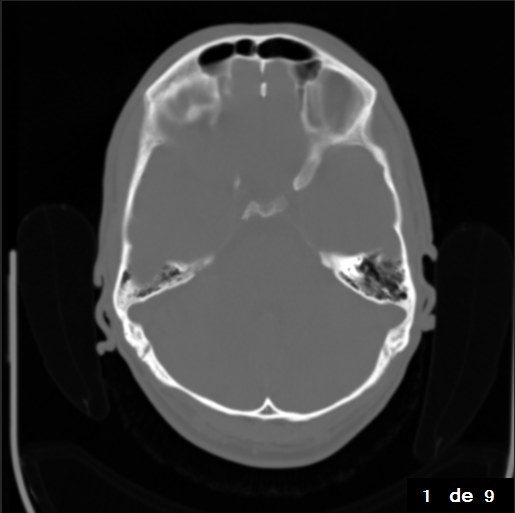
\includegraphics[width = 7 cm, height = 7 cm]{contrasteDefault}
\caption{TAC con un contraste completo.}
Captura de pantalla del sistema en funcionamiento.
\end{figure}

\begin{figure}[H]
\centering
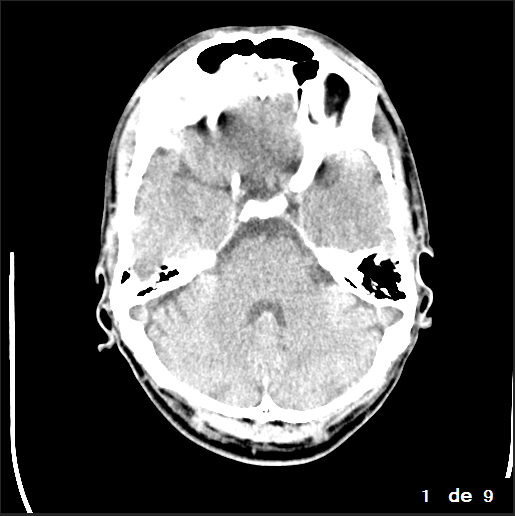
\includegraphics[width = 7 cm, height = 7 cm]{contrasteCerebro}
\caption{TAC con el contraste recomendado para cerebro.}
Captura de pantalla del sistema en funcionamiento.
\end{figure}

\begin{figure}[H]
\centering
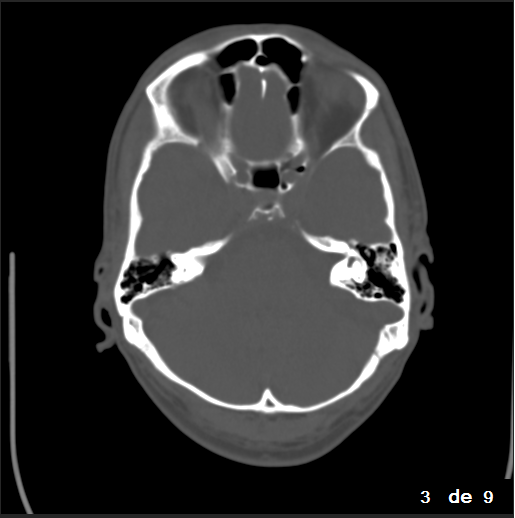
\includegraphics[width = 7 cm, height = 7 cm]{contrasteHueso}
\caption{TAC con el contraste recomendado para hueso.}
Captura de pantalla del sistema en funcionamiento.
\end{figure}

\begin{figure}[H]
\centering
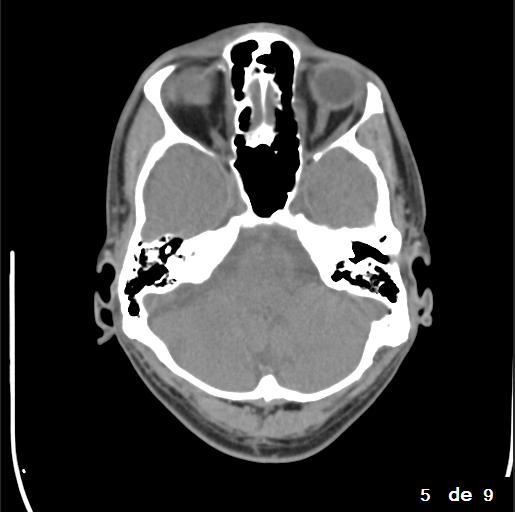
\includegraphics[width = 7 cm, height = 7 cm]{contrasteParteBlandas}
\caption{TAC con el contraste recomendado para partes blandas.}
Captura de pantalla del sistema en funcionamiento.
\end{figure}

\begin{figure}[H]
\centering
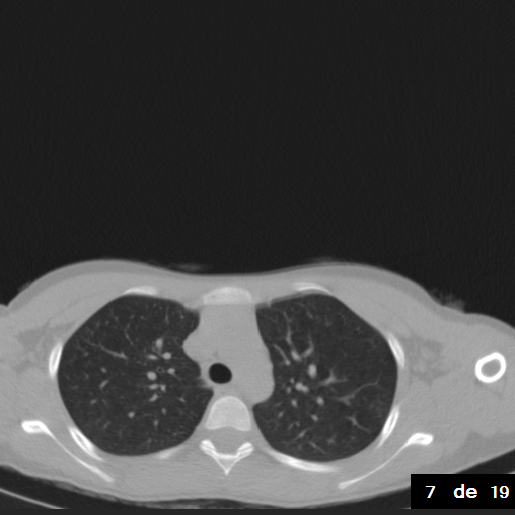
\includegraphics[width = 7 cm, height = 7 cm]{contrastePulmon}
\caption{TAC con el contraste recomendado para pulmón.}
Captura de pantalla del sistema en funcionamiento.
\end{figure}

\section{Clasificadores}
A continuación se muestran los resultados obtenidos con las técnicas de clasificación utilizadas.\\

La técnica Fuzzy C-Means se implementa sobre una TAC en la zona abdominal donde podemos encontrar una gran acumulación de diferentes tejidos. Se pueden observar los valores máximos y mínimos de cada grupo y el color con el que está representado. Adicionalmente se puede observar la implementación de la herramienta de zoom para ver con más detalles algunos tejidos.

\vspace{1cm}
\begin{figure}[H]
\centering
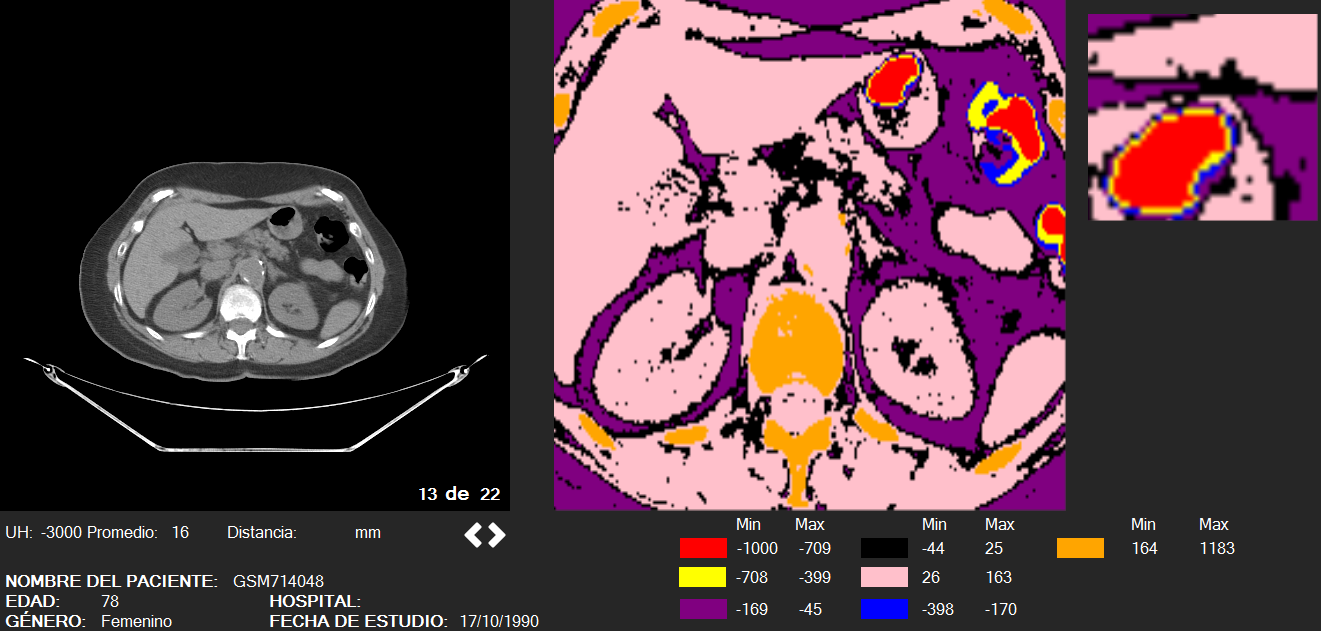
\includegraphics[width = 15 cm, height = 10 cm]{clusterCfuzzy}
\caption{Algoritmo Fuzzy C-Means aplicado a una TAC.}
Captura de pantalla del sistema en funcionamiento.
\end{figure}

\newpage
\vspace*{3cm}
La técnica K-Means se implementa sobre una TAC de la zona torácica.
\begin{figure}[H]
\centering
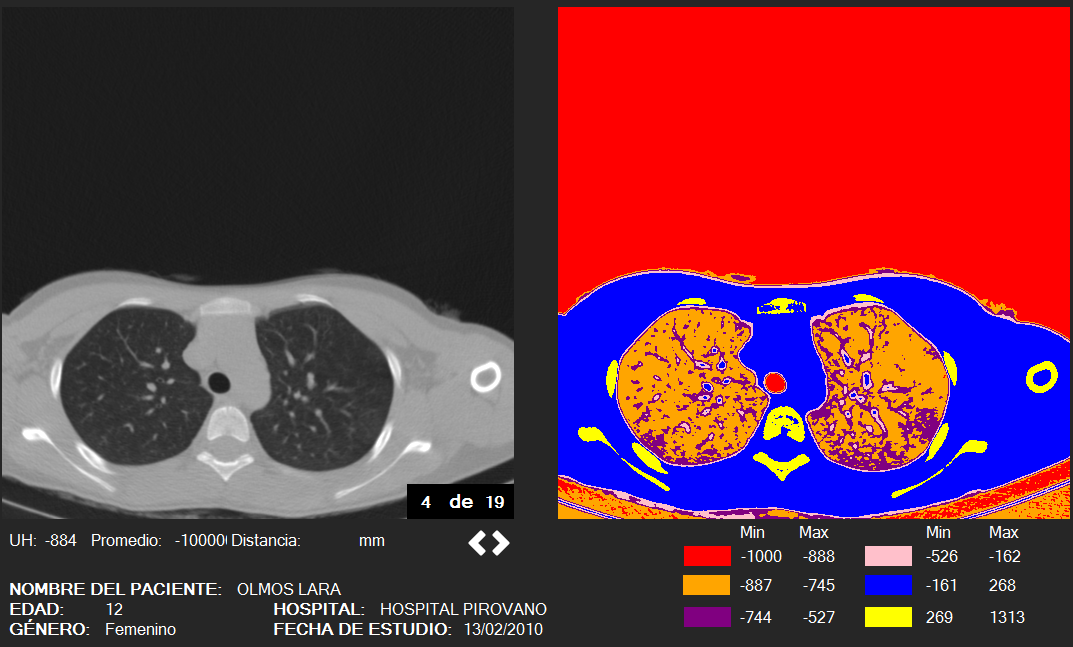
\includegraphics[width = 15 cm, height = 10 cm]{clusterKmeans}
\caption{Algoritmo K-Means aplicado a una TAC.}
Captura de pantalla del sistema en funcionamiento.
\end{figure}

\section{Segmentación}
La técnica de Región creciente se implementa sobre una TAC de zona abdominal y intenta aislar organos de hueso y fluidos.
\vspace*{3cm}
\begin{figure}[H]
\centering
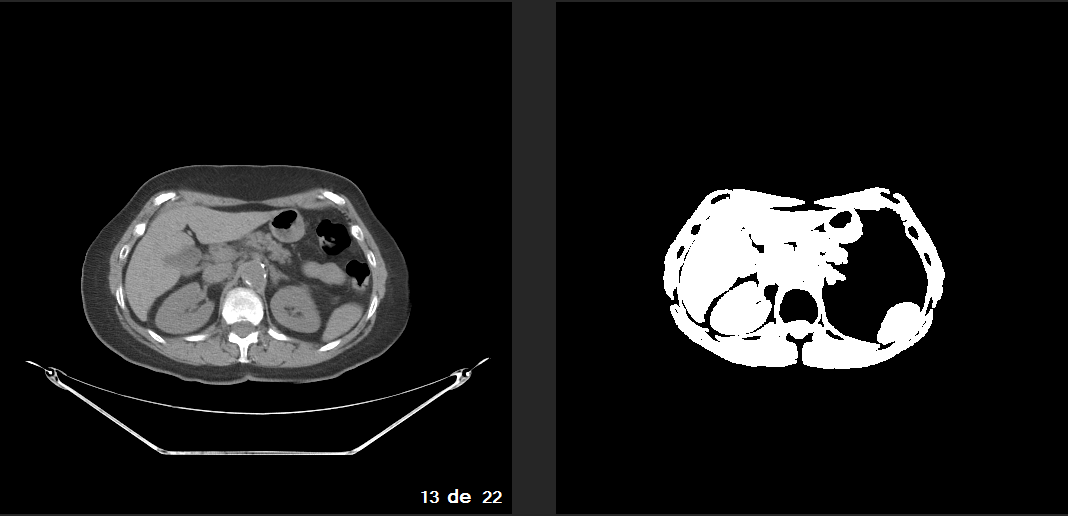
\includegraphics[width = 15 cm, height = 10 cm]{segmentacionRegionCreciente}
\caption{Región creciente en zona abdominal.}
Captura de pantalla del sistema en funcionamiento.
\end{figure}



\chapter{Conclusiones y trabajo futuro}
\section{Conclusiones}
Una vez terminado el sistema se llegó a las siguientes conclusiones:
\begin{itemize}
\item Se cumplieron los objetivos planteados para el desarrollo del sistema.
\item La extensión del sistema cubre aspectos que las herramientas actuales no proporcionan sin embargo sigue siendo una herramienta de menor nivel que los softwares ofrecidos en los equipos médicos especializados.
\item El hacer una implementación propia de los algoritmos nos ayudó pues pudimos orientarlos a nuestra arquitectura y hacer un manejo integro de los datos, quitando las limitaciones que en muchas ocasiones tienen las librerías.
\item Cuando el especialista encuentra incongruencias dentro de la TAC el uso de técnicas no supervisadas puede ser muy útil como una segunda opinión de los resultados obtenidos.
\end{itemize}


\section{Trabajo a futuro}
Las propuestas de trabajo futuro para este sistema son las siguientes:
\begin{itemize}
\item Incluir más técnicas de clasificación y segmentación para el análisis de TAC.
\item Implementar métodos exploratorios en las TAC.
\item Hacer una implementación propia para la representación en 3D de TAC.
\item Incluir un módulo de comparación entre las tomografías analizadas e hsitóricos de la medicina.
\item Agregar más herramientas que faciliten el manejo de las TAC y complementen el análisis.
\item Permitir al especialista observar todos los campos disponibles en la cabecera del archivo DICOM.
\item Desarrollar una API de la aplicación para permitir su uso a terceros.
\end{itemize}

\appendix
\chapter{Código K-Means}

Esta función genera centros aleatorios.
\lstset{language=C, breaklines=true, basicstyle=\footnotesize}
\lstset{numbers=left, numberstyle=\tiny, stepnumber=1, numbersep=-2pt}
\begin{lstlisting}[frame=single]
	public void generarCentros(){
            centros = new List<Double>();
            rnd = new Random();
            for (int i = 0; i < numerosK; i++) {
                int numero = rnd.Next((IgnorarAire ? IGNORAR : -1000), 1400);
                centros.Add((double)numero);
            }
        }
\end{lstlisting}

\vspace*{1cm}
Esta función Euclidiana entre dos densidades. 
\lstset{language=C, breaklines=true, basicstyle=\footnotesize}
\lstset{numbers=left, numberstyle=\tiny, stepnumber=1, numbersep=-2pt}
\begin{lstlisting}[frame=single]
	public void distanciaEuclidiana(int i, int j){
            if (IgnorarAire && datos[i][j] < IGNORAR) return;
            int indc = 0;
            conjunto.Clear();
            foreach (Double indice in centros){
                Double resta = Math.Abs(datos[i][j] - indice);
                conjunto.Add(resta);
            }
            for (int k = 1; k < conjunto.Count; k++)
                if (conjunto[indc] > conjunto[k])
                    indc = k;
            clases[i, j] = indc + 1;
        }
\end{lstlisting}

\newpage
La función promedio saca el promedio de las densidaes en el cluster y genera nuevos centros con base en el promedio calculado.
\lstset{language=C, breaklines=true, basicstyle=\footnotesize}
\lstset{numbers=left, numberstyle=\tiny, stepnumber=1, numbersep=-2pt}
\begin{lstlisting}[frame=single]
	public void promedio(){
            centros.Clear();
            double[] sumas = new double[numerosK];
            double[] contador = new double[numerosK];
            for (int i = 0; i < numerosK; i++)            
                sumas[i] = contador[i] = 0;            
            for (int i = 0; i < datos.Count; i++){
                for (int j = 0; j < datos[i].Length; j++){
                    if (IgnorarAire && datos [i] [j] < IGNORAR)
                        continue;
                    sumas[clases[i, j] - 1] += datos[i][j];
                    contador[clases[i, j] - 1]++;
                }
                if (reporte_progreso.CancellationPending)
                    return;
                operaciones_cargando++;
                reporte_progreso.ReportProgress((90 * operaciones_cargando) / operaciones_total);
            }
            centros.Clear();
            for (int i = 0; i < numerosK; i++) {
                if (contador [i] == 0) {
                    centros.Add(ObtenPixelRandom());
                } else {
                    centros.Add(sumas [i] / contador [i]);
                }
            }
            
        }
\end{lstlisting}

\chapter{Código Fuzzy C-Means}
Se generan los centros aleatorios.
\lstset{language=C, breaklines=true, basicstyle=\footnotesize}
\lstset{numbers=left, numberstyle=\tiny, stepnumber=1, numbersep=-2pt}
\begin{lstlisting}[frame=single]
	public void generarCentros(){
            centros = new List<Double>();
            rnd = new Random();
            for (int i = 0; i < numerosK; i++) {
                int numero = rnd.Next((IgnorarAire ? IGNORAR : -1000), 1400);
                centros.Add((double)numero);
            }
        }
\end{lstlisting}

\vspace*{1cm}
Se calcula la distancia con base a la diferencia de densidades.
\lstset{language=C, breaklines=true, basicstyle=\footnotesize}
\lstset{numbers=left, numberstyle=\tiny, stepnumber=1, numbersep=-2pt}
\begin{lstlisting}[frame=single]
	public void GenerarDistancias(){
            for (int i = 0; i < N; i++){
                if (reporte_progreso.CancellationPending)
                    return;
                for (int j = 0; j < M; j++){
                    if (IgnorarAire && datos [i] [j] < IGNORAR)
                        continue;
                    for (int k = 0; k < numerosK; k++){
                        double dist = datos[i][j] - centros[k];
                        distancias[i, j, k] = dist * dist;
                    }
                }
            }
        }
\end{lstlisting}

\newpage
\vspace*{3cm}
Se crea la matriz de pertenencia, dando un valor de pertenencia a cada densidad para cada cluster.
\lstset{language=C, breaklines=true, basicstyle=\footnotesize}
\lstset{numbers=left, numberstyle=\tiny, stepnumber=1, numbersep=-2pt}
\begin{lstlisting}[frame=single]
	public void ActualizarPertenencia(){
            for (int i = 0; i < N; i++){
                operaciones_cargando++;
                reporte_progreso.ReportProgress((operaciones_cargando * 90) / operaciones_total);
                if (reporte_progreso.CancellationPending)
                    return;
                for (int j = 0; j < M; j++){
                    if (IgnorarAire && datos [i] [j] < IGNORAR)
                        continue;
                    for (int k = 0; k < numerosK; k++){
                        double sum = 0.0;
                        for (int l = 0; l < numerosK; l++)
                            sum += Math.Pow(distancias[i, j, k] / distancias[i, j, l], 2.0 / (m - 1.0));  
                        pertenencia[i, j, k] = 1.0 / sum;
                            
                    }
                    
                }
            }
        }
\end{lstlisting}

\newpage
\vspace*{2cm}
Se generan los nuevos centros para las iteraciones siguientes.
\lstset{language=C, breaklines=true, basicstyle=\footnotesize}
\lstset{numbers=left, numberstyle=\tiny, stepnumber=1, numbersep=-2pt}
\begin{lstlisting}[frame=single]
	public void GeneraNuevosCentros(){
            for (int k = 0; k < numerosK; k++){
                long aa = 0;
                long bb = 0;
                for (int p = 0; p < N; p++){
                    if (reporte_progreso.CancellationPending)
                        return;
                    for (int i = 0; i < M; i++){
                        if (IgnorarAire && datos [p][i] < IGNORAR)
                            continue;
                        double valor = Math.Round(Math.Pow(pertenencia[p, i, k], m), 5);
                        if (valor <= 0.00001)
                            continue;
                        aa += (long)(Math.Round(valor * datos[p][i], 5) * 100000);
                        bb += (long)(valor * 100000);
                        
                    }
                }
                if (bb <= 0.0001) {
                    centros [k] = ObtenPixelRandom();
                } else {
                    centros [k] = (double)aa / (double)bb;
                }
            }
        }
\end{lstlisting}

\chapter{Diagrama de clases}

La siguiente imagen muestra las clases utilizadas en el sistema. El paradigma de la programación orientada a objetos nos ayudó a llevar un mejor control sobre los diferentes algoritmos y herramientas implementadas.
\newpage
\begin{figure}[H]
\centering
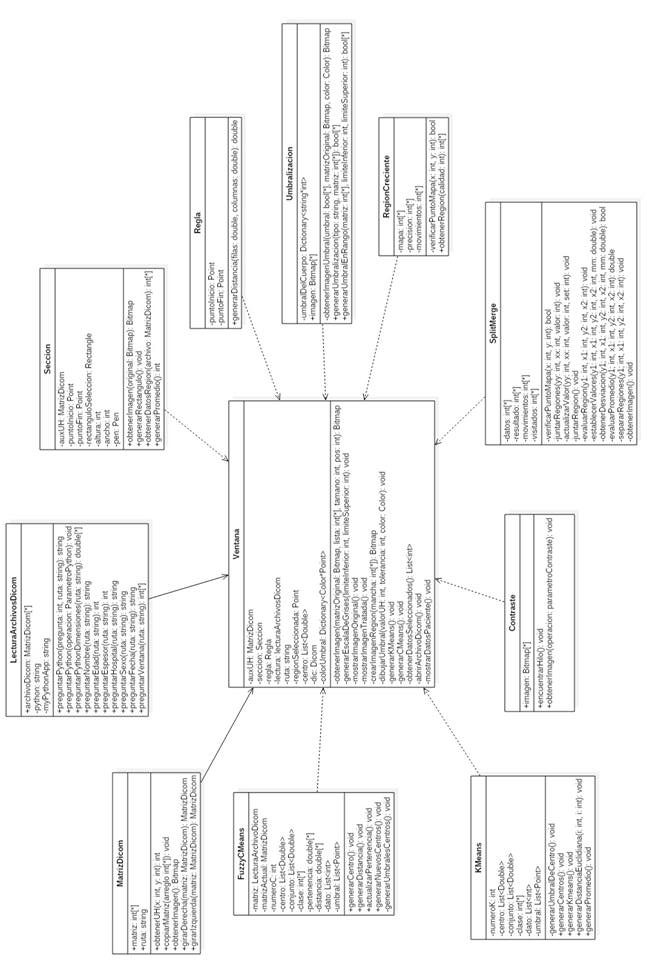
\includegraphics[width = 15 cm, height = 18 cm]{diagramaClases}
\caption{Diagrama de clases del sistema.}
Imagen de elaboración propia.
\end{figure}

\bibliographystyle{IEEEtran}
\bibliography{bibliografia}

\end{document}
